\documentclass[5p,twocolumn,authoryear]{elsarticle}
\usepackage[T1]{fontenc}
\usepackage{lmodern}
\setlength{\emergencystretch}{1em}
\usepackage{amsmath,amssymb,booktabs,graphicx,array,microtype}
\usepackage{xcolor,hyperref}
\usepackage{dblfloatfix}
\renewcommand{\topfraction}{0.95}
\renewcommand{\dbltopfraction}{0.95}
\renewcommand{\textfraction}{0.05}
\renewcommand{\floatpagefraction}{0.75}
\renewcommand{\dblfloatpagefraction}{0.75}
\setcounter{dbltopnumber}{2}
\usepackage{tikz}
\usetikzlibrary{arrows.meta,positioning,fit,backgrounds}
\hypersetup{colorlinks=true,linkcolor=blue!50!black,citecolor=blue!50!black,urlcolor=blue!50!black}
\newcommand{\todo}[1]{\textcolor{red!70!black}{[TO COMPLETE: #1]}}
\newcommand{\nojepa}{\textsc{NoJEPA}}
\newcommand{\direct}{\textsc{DirectReadout}}
\newcommand{\fullmodel}{\textsc{ForecastAttention}}
\newcommand{\meanmodel}{\textsc{ForecastMean}}
\journal{Medical Image Analysis}
\begin{document}
\begin{frontmatter}
\title{Forecast-aware latent modeling for longitudinal prediction of pathological complete response from breast MRI}
\author{Author information to be completed}
\address{Affiliations and corresponding author to be completed}
\begin{abstract}
Longitudinal breast MRI can reveal treatment response, but endpoint classifiers do not explicitly model the future trajectory implied by an observed history. We investigate forecast-aware latent modeling for pathological complete response (pCR) prediction using three-phase dynamic contrast-enhanced MRI, baseline clinical variables, and assigned-arm scenarios. An autonomous predictor estimates future latent states, and an attention readout combines the predicted terminal state, its change, and direct history features. The cohort comprises 976 patients and 3,641 examinations, with 801 development patients and a fixed internal holdout of 175 patients, including 56 positive outcomes. Three matched variants compare prediction without future-state supervision, auxiliary-supervised direct prediction, and forecast-attention readout. Each variant uses training seed 44; five fold probabilities are averaged per patient before computing metrics. The complete model achieved T0/T1/T2 AUROCs of 0.7450/0.7521/0.7550 and macro AUROC/AP/F1 of 0.7507/0.6283/0.5604, compared with 0.7279/0.5968/0.5416 for the control without future-state supervision. Auxiliary-supervised direct readout had higher macro F1 (0.5678), and a supplementary mean-pooling model reached 0.5742. Expanded analysis revealed lower macro specificity and worse probability quality for the complete model, threshold-dependent net benefit, and uncertain subgroup differences. Archived training probes did not show uniformly better latent forecasting. The complete-versus-control macro AUROC difference had nominal paired DeLong $p=0.0462$ and Holm-adjusted $p=0.4161$; none of the nine principal comparisons met the adjusted significance criterion. These exploratory findings require independent validation; the seed and ensemble policy were selected retrospectively.
\end{abstract}
\begin{keyword}
Breast MRI \sep Pathological complete response \sep Longitudinal imaging \sep Latent dynamics \sep Treatment response prediction
\end{keyword}
\end{frontmatter}
\section{Introduction}
\label{sec:intro}
Neoadjuvant systemic therapy provides an opportunity to monitor breast cancer before surgery and to study how an individual tumor responds over time. Pathological complete response (pCR) is a clinically meaningful endpoint associated with long-term outcomes, although its relationship to prognosis varies across biological subtypes and it should not be equated with a universally valid trial-level surrogate \citep{ctneobc2014}. Predicting pCR from imaging could support response assessment and the design of future adaptive studies. Such a prediction remains a prognostic estimate under an observed treatment context; it does not establish that changing treatment would improve an individual patient's outcome.

Dynamic contrast-enhanced MRI captures three-dimensional anatomy and contrast uptake patterns that evolve during therapy. Prior work in the I-SPY setting has demonstrated associations between MRI-derived tumor measurements and pathological response or subsequent outcomes \citep{hylton2012mri,hylton2016ftv}. Public multicenter imaging resources also make it possible to examine learned representations across repeated visits \citep{tciaispy2_2022,tciaacrin6698_2021}. However, a longitudinal prediction system must operate at the time a decision is considered: a baseline prediction can use baseline information, whereas an interim prediction can use the examination history accumulated by that interim visit. Future scans may inform representation learning on development patients but cannot become inputs to predictions for holdout patients at an earlier landmark.

Most direct classifiers optimize the endpoint of interest from observed images and clinical variables. This is a reasonable objective, but it does not explicitly require the representation to capture how the tumor state may evolve. A different strategy is to predict future imaging information and use the prediction to inform the endpoint readout. Image synthesis provides one route to such a representation, but prediction in a compact latent space can focus the training signal on state evolution without requiring a pixel-space image generator at inference. This distinction is useful for response prediction: the relevant question is whether the learned forecast contributes information to classification, rather than whether a generated image is visually convincing.

Joint-embedding predictive learning offers a general mechanism for predicting target representations computed by a slowly updated encoder \citep{jepa2023}. In a longitudinal medical setting, adapting that principle requires explicit handling of partial histories, missing future observations, treatment context, and the distinction between an auxiliary training target and a classifier input. A model may benefit from a future-state loss while still making a direct prediction from the observed history. Conversely, directly including forecast features in the classifier changes both its information pathway and its parameterization. These effects should be examined through matched controls rather than attributed to a single generic ``world model'' component.

We investigate forecast-aware latent modeling for longitudinal pCR prediction from breast MRI. The model encodes three selected DCE phases at each available visit, fuses observed MRI with baseline clinical information and an assigned treatment-arm scenario, and autonomously rolls the current latent state forward to a terminal stage. A spatial attention mechanism summarizes the predicted terminal state and the predicted change from the current state for pCR classification. We compare the complete model with two direct-readout controls: one without future-state supervision and one with the same auxiliary supervision as the complete model. A supplementary mean-pooling model further examines the attention component.

The study makes three concrete contributions. First, it formulates a common representation and masked future-state objective that can be applied to available T0--T2 histories while using observed later scans only as development-time targets. Second, it provides a staged comparison that distinguishes the effect of auxiliary prediction from the joint effect of forecast readout and attention. Third, it reports landmark-specific discrimination, class-specific errors, calibration, hypothetical decision curves, subgroup heterogeneity, archived forecasting diagnostics, and paired patient-level uncertainty on a fixed internal holdout. The manuscript evaluates each variant as a seed-44 ensemble, averaging five fold probabilities for each patient before computing metrics. This seed and aggregation policy was chosen retrospectively; the analysis remains exploratory, with seed-selection and upstream-independence limits stated explicitly.

\section{Related work}
\label{sec:related}
\paragraph{MRI biomarkers and learned pCR prediction.}
MRI-based response assessment has a substantial clinical and quantitative foundation. Functional tumor volume and related measurements have been studied in longitudinal breast MRI cohorts, including I-SPY \citep{hylton2012mri,hylton2016ftv}. The ACRIN 6698 study additionally examined diffusion-derived measurements in relation to response \citep{ACRIN6698diffusion2018}. These studies motivate imaging-based monitoring but do not establish that a learned model using different inputs or a different evaluation split has equivalent clinical validity. Our experiments use selected DCE phases and baseline clinical variables; diffusion imaging is not an input to the present model.

Learning-based approaches can combine complementary image sequences or repeated examinations. Synthesis-based representation learning has been explored for multi-sequence 3D/4D MRI \citep{han2024synthesis}, and recent studies have examined spatiotemporal or early-treatment information for pCR prediction \citep{tang2025spatiotemporal,du2025early}. Such studies provide relevant methodological context, but differences in patient selection, imaging availability, endpoints, and holdout construction prevent direct numerical comparisons with our results. We therefore do not claim superiority to published systems from cross-paper metric comparisons. Reimplementation of suitable external baselines under the same patient split remains necessary.

\paragraph{Predictive latent representations.}
Predicting a target embedding rather than reconstructing the input image is a central idea in joint-embedding predictive learning \citep{jepa2023}. We use an exponential-moving-average target encoder to define latent states and supervise autonomous future predictions. The present objective is a supervised pCR loss combined with a masked multi-step latent-state loss. It does not activate a separate single-step teacher-forcing JEPA loss, image reconstruction loss, or latent-variance regularizer. This objective-level distinction matters when interpreting the internal experiment name \nojepa{}: that control removes future-state supervision, while retaining the common fusion architecture.

\paragraph{Attention and volumetric image representation.}
Transformer attention provides a flexible way to combine image tokens and contextual information \citep{vaswani2017}. Compact convolutional representations can reduce the cost of processing volumetric MRI, and vector-quantized generative models provide one source of pretrained convolutional encoders \citep{vqgan2021}. Here the pretrained codec contributes a continuous convolutional encoder. The quantizer and image decoder are bypassed, and the main experiments do not synthesize MRI volumes. The final attention weights summarize latent tokens that have already undergone spatial mixing; they are therefore not validated lesion segmentations or anatomical explanations.

\section{Method}
\label{sec:method}
\begin{figure*}[t]
\centering
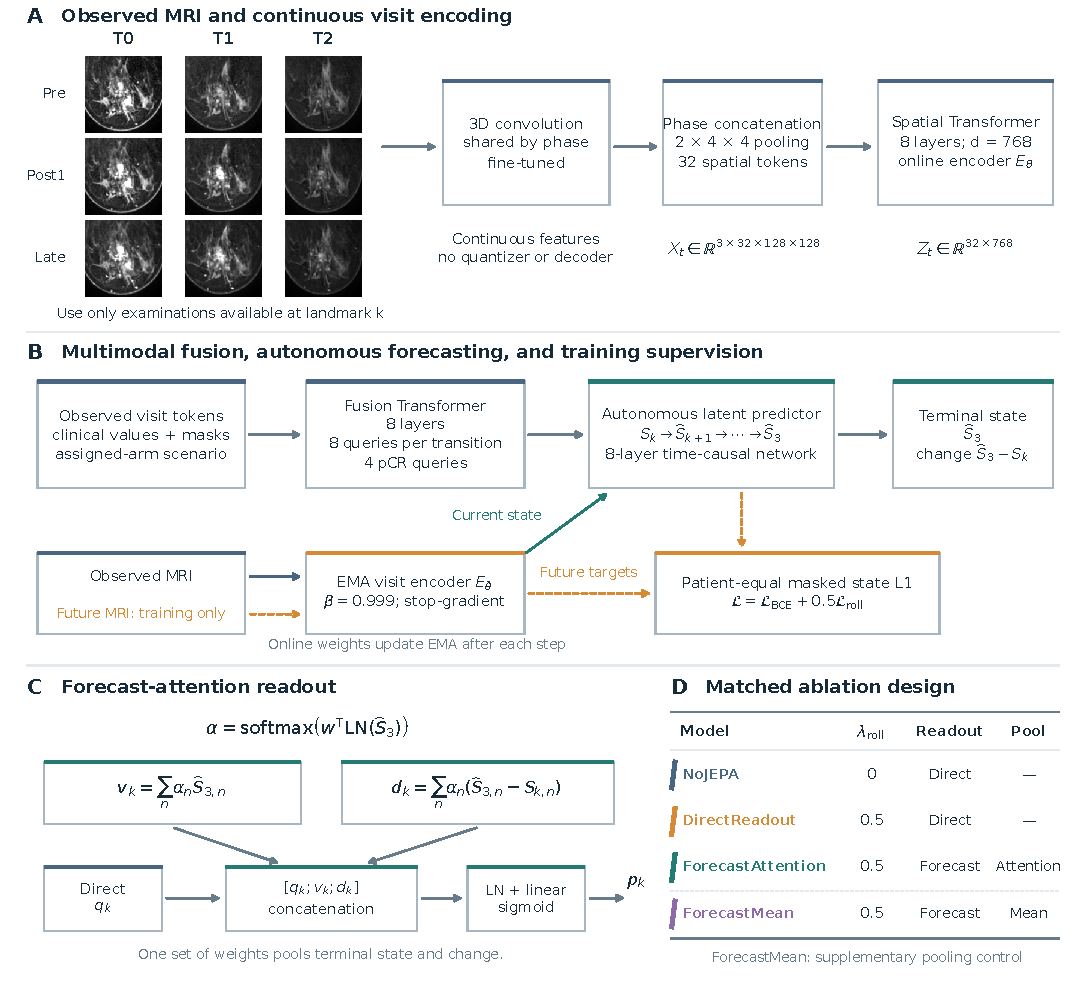
\includegraphics[width=\textwidth]{figures/framework.pdf}
\caption{Forecast-aware latent modeling and matched controls. (A) Real three-phase MRI crops from one development patient illustrate the same baseline-defined plane at T0, T1, and T2; the example and slice were selected without outcomes or pCR predictions. Only visits available at the prediction landmark are inputs. A shared continuous encoder and spatial Transformer produce visit tokens. (B) Clinical values, availability masks, and an assigned-arm scenario condition fusion and autonomous prediction to T3. The EMA encoder supplies the detached current state; available future MRI supplies training targets only. Dashed orange arrows denote training-target or loss paths. (C) Attention weights pool the predicted terminal state and its change; these features are combined with direct pCR-query features. (D) The primary variants separate removal of future-state supervision from the complete forecast readout. ForecastMean is a supplementary pooling control. One fold model is illustrated; evaluation averages the five seed-44 fold probabilities per patient. MRI tiles are illustrative crops, not generated images, segmentation ground truth, or attention maps.}
\label{fig:framework}
\end{figure*}


\subsection{Longitudinal prediction problem}
\label{sec:problem}
We consider prediction of pathological complete response (pCR) from a patient's available magnetic resonance imaging (MRI) history during neoadjuvant treatment. Canonical examination stages are indexed by $t\in\{0,1,2,3\}$. At a prediction landmark $k\in\{0,1,2\}$, the model receives only examinations acquired and available by that landmark. Let $X_t\in\mathbb{R}^{3\times32\times128\times128}$ denote the processed examination at stage $t$, and let $o_t^{(k)}$ indicate whether this examination is available in the observed prefix. Missing examinations retain their canonical stage rather than shifting later examinations forward. The three channels contain the pre-contrast acquisition, the first post-contrast acquisition, and a metadata-selected late post-contrast acquisition, respectively. The late acquisition is not assumed to have the same acquisition index for all examinations.

The observed information is
\begin{equation}
 \mathcal{H}_k=\bigl\{(X_t,t):o_t^{(k)}=1\bigr\}\cup
 \bigl\{c_k,m_k,a_k,\tau_k\bigr\},
\end{equation}
where $c_k\in\mathbb{R}^{4}$ contains the available clinical variables, $m_k$ their availability indicators, $a_k$ the available assigned treatment-arm category, and $\tau_k$ its declared availability stage. The clinical variables are age at screening, hormone-receptor positivity, HER2 positivity, and a binary MammaPrint variable. Age is standardized using the current training partition; binary variables retain their original coding. Unavailable values are set to zero after standardization and accompanied by an explicit mask. The clinical token embeds the concatenated values and masks. Treatment conditioning uses 13 released arm categories and an additional unknown category. In this retrospective experiment, assigned arm and available baseline clinical variables are assumed to be known at T0. This is an assigned-arm scenario; the categorical input does not specify actual doses, treatment intervals, or treatment changes, and it does not support a causal interpretation.

The output is $p_k=\Pr(y=1\mid\mathcal{H}_k)$, where $y\in\{0,1\}$ is the final pCR label. Future MRI is stored separately as training supervision and is excluded from the prediction input. T3 can provide a future representation target during training, but is never a prediction landmark in the reported T0--T2 protocol.

\subsection{Continuous MRI encoding and multimodal fusion}
\label{sec:encoding}
Each observed examination is encoded independently by an online visit encoder $E_{\theta}$. Its convolutional front end shares the same single-channel weights across the three acquisition phases. Two stride-two three-dimensional convolutional stages, residual blocks, and group normalization produce 64 continuous feature channels per phase at one-quarter input resolution along each spatial axis. The three phase-specific feature maps are concatenated, adaptively averaged to a $2\times4\times4$ grid, and projected to a latent width of $d=768$. This gives $N=32$ spatial tokens per examination. Learned spatial positional embeddings and an eight-layer spatial Transformer then produce the visit representation $Z_t=E_{\theta}(X_t)\in\mathbb{R}^{N\times d}$.

The convolutional front end is initialized from the same pre-existing VQ-GAN-style codec checkpoint for all compared models and is fine-tuned. Here, the model uses continuous features from the codec encoder before its compression projection. It does not use discrete codebook assignments, a quantization objective, a decoder, or adversarial learning during downstream pCR training. \todo{Document the original codec pretraining dataset, patient-level overlap with the present partitions, checkpoint provenance, and applicable redistribution terms.}

Stage embeddings distinguish examination times. Observed image tokens, one clinical token, and one treatment-arm token form the multimodal context. An eight-layer fusion Transformer additionally receives eight learned transition-query tokens for each of the three canonical transitions and four pCR-query tokens. Transition-query slots are retained at every landmark, independently of which future targets happen to be available. Their conditioning is derived entirely from the observed prefix. Context tokens interact bidirectionally; appended transition and pCR queries use a causal attention mask and can attend to the context and preceding query positions. Padding masks remove unobserved image tokens. This produces transition features $A_{j+1}^{(k)}\in\mathbb{R}^{8\times d}$ for transitions $j\rightarrow j+1$, and pCR-query features $Q_k\in\mathbb{R}^{4\times d}$.

All spatial, fusion, and prediction Transformers use pre-normalization blocks, GELU feed-forward layers of width 3072, and dropout 0.3, following the attention-based architecture of \citet{vaswani2017}. Attention has 16 heads with 64 channels per head: its internal width is therefore 1024, followed by projection back to the 768-dimensional residual stream. The clinical and treatment tokens condition forecasting through the shared fusion network rather than through a separately supplied future treatment trajectory.

\subsection{EMA target states and autonomous forecasting}
\label{sec:forecasting}
A target visit encoder $E_{\bar\theta}$ is initialized as a copy of the online encoder and updated after each optimizer step by exponential moving average (EMA):
\begin{equation}
 \bar\theta\leftarrow\beta\bar\theta+(1-\beta)\theta,
 \qquad \beta=0.999.
\end{equation}
The target encoder remains in evaluation mode and receives no gradients. It defines a common representation space for the observed initial state and available future targets,
\begin{equation}
 S_t=\operatorname{stopgrad}\!\left(E_{\bar\theta}(X_t)\right)
 \in\mathbb{R}^{N\times d}.
\end{equation}
Encoding a future target in this branch supplies a loss target only; it does not make that examination available to the forecasting or classification input.

The predictor starts from the latest actually observed state in $\mathcal{H}_k$ and recursively advances to T3. For the reported landmarks, this initial state is $S_k$. At each future transition, it uses the corresponding transition features and its previously generated states. A history input additionally embeds the difference between a source state and its latest available predecessor, with a separate indicator for whether a predecessor exists. Observed history is used where available; after the landmark, the history is extended using model predictions. Thus, a missing future examination removes supervision at that time but does not interrupt the simulated transition sequence.

The prediction network is an eight-layer time-causal Transformer. Each transition block contains its eight transition tokens and 32 spatial source-state tokens, together with learned spatial and temporal embeddings. Tokens can interact within a block; attention between transition blocks is directed from earlier to later blocks. A learned root token remains available when some blocks are masked. The network predicts a residual state increment,
\begin{equation}
 \widehat S_{j+1}=\widetilde S_j+
 G_{\phi,j}\!\left(\widetilde S_{k:j},A_{k+1:j+1}^{(k)},D_{k:j}\right),
 \qquad j=k,\ldots,2,
\end{equation}
where $\widetilde S_k=S_k$, subsequent $\widetilde S_j$ are generated states, and $D_{k:j}$ denotes the available predecessor differences and validity indicators. The residual output projection is initialized to zero, so prediction initially preserves the source state. The transition features summarize the complete legal prefix even when only a subset of previous state differences is available to a particular prediction block.

Forecasts are generated autonomously during training and inference. A true future state never replaces a predicted predecessor. The classifier likewise uses this autonomous trajectory. The configuration includes no teacher-forced next-state loss in these experiments. EMA encoding of real future examinations is used exclusively to evaluate representation error against available targets.

\subsection{Prediction-conditioned pCR readout}
\label{sec:readout}
The full model, \fullmodel{}, combines a direct summary of the observed prefix with summaries of the predicted terminal state and its change from the current state. First, the four pCR-query features are averaged to obtain $q_k=\frac14\sum_{r=1}^{4}Q_{k,r}$. For spatial token $n$, the forecast change is $\Delta S_{k,n}=\widehat S_{3,n}-S_{k,n}$. A learned scalar scorer defines
\begin{equation}
 \alpha_{k,n}=
 \frac{\exp\!\left(w^{\mathsf T}\operatorname{LN}(\widehat S_{3,n})\right)}
 {\sum_{u=1}^{N}\exp\!\left(w^{\mathsf T}\operatorname{LN}(\widehat S_{3,u})\right)}.
\end{equation}
The same weights pool terminal state and change,
\begin{equation}
 v_k=\sum_{n=1}^{N}\alpha_{k,n}\widehat S_{3,n},
 \qquad
 d_k=\sum_{n=1}^{N}\alpha_{k,n}\Delta S_{k,n}.
\end{equation}
The final prediction is
\begin{equation}
 p_k=\sigma\!\left(b+u^{\mathsf T}
 \operatorname{LN}\!\left([q_k;v_k;d_k]\right)\right).
\end{equation}
The scorer is initialized with $w=0$, corresponding to uniform pooling at initialization. Classification gradients propagate through the generated terminal state, predictor, and transition-conditioning pathway. The observed EMA reference state remains detached. The attention weights summarize transformed spatial tokens and should not be interpreted as validated anatomical localization or tumor segmentation.

For \direct{}, pCR is instead predicted directly from $q_k$ using a layer-normalized linear head. Its future-state predictor is trained as an auxiliary task, but generated states are not explicit inputs to the pCR head. The direct head has input width $d$, whereas the full readout has width $3d$. Their comparison therefore evaluates the complete forecast-conditioned readout, including its state and change inputs and classifier width. An additional mean-pooling variant, when reported, retains the forecast-conditioned readout and replaces $\alpha_{k,n}$ by $1/N$.

\subsection{Training objective and matched ablations}
\label{sec:objective}
Let $\mathcal{B}_{y}$ be the labeled patients in a training batch, and let $m_{i,t}^{\mathrm{future}}$ indicate an actually available future target for patient $i$ after its sampled landmark. The pCR objective is unweighted binary cross-entropy,
\begin{equation}
 \mathcal{L}_{\mathrm{pCR}}=
 -\frac{1}{|\mathcal{B}_{y}|}\sum_{i\in\mathcal{B}_{y}}
 \left[y_i\log p_i+(1-y_i)\log(1-p_i)\right].
\end{equation}
Define $M_i=\sum_t m_{i,t}^{\mathrm{future}}$ and $\mathcal{B}_{+}=\{i:M_i>0\}$. Autonomous representation supervision is patient-equal:
\begin{equation}
 \mathcal{L}_{\mathrm{roll}}=
 \frac{1}{|\mathcal{B}_{+}|}\sum_{i\in\mathcal{B}_{+}}
 \frac{1}{M_i}\sum_t m_{i,t}^{\mathrm{future}}
 \frac{\|\widehat S_{i,t}-S_{i,t}\|_1}{Nd}.
\end{equation}
If a batch contains no future targets, this term is zero. Each available future examination has equal weight within a patient; the loss uses no horizon discount, lesion weighting, or fabricated target for a missing visit. Patients without future MRI still contribute pCR supervision.

The full model and \direct{} minimize
\begin{equation}
 \mathcal{L}=\mathcal{L}_{\mathrm{pCR}}+0.5\mathcal{L}_{\mathrm{roll}}.
\end{equation}
\nojepa{} uses the direct pCR head with $\mathcal{L}=\mathcal{L}_{\mathrm{pCR}}$. This historical control name denotes removal of future-state auxiliary supervision, rather than removal of every transition-related module: it retains the shared fusion architecture and transition-query slots. Consequently, \direct{} versus \nojepa{} isolates the added autonomous representation objective under the same direct readout, whereas \fullmodel{} versus \direct{} assesses the added forecast-conditioned classification pathway. The latter comparison cannot isolate spatial attention alone.

All three models omit teacher-forced JEPA, image reconstruction, flow-matching, and variance-regularization losses. In particular, the future objective reported here is autonomous state prediction, despite the JEPA-related implementation lineage. During training, patients are shuffled once per epoch and one actual available T0--T2 landmark is sampled uniformly for each patient. This balances patient contributions without treating a patient with more visits as several independently sampled patients. The same clinical endpoint supervises each sampled prefix; validation assesses all available eligible prefixes using patient-equal weighting.

\section{Dataset and preprocessing}
\label{sec:data}

\subsection{Cohort construction and clinical variables}
We retrospectively analysed longitudinal breast dynamic contrast-enhanced MRI
(DCE-MRI) from the public I-SPY2 and ACRIN-6698 imaging
resources~\cite{tciaispy2_2022,tciaacrin6698_2021}. Source imaging identifiers
were linked to research identifiers using the accompanying official identity
mapping, and outcomes and baseline clinical variables were obtained from the
official I-SPY2 Imaging Cohort~1 clinical spreadsheet. The final cohort
comprised 976 patients with 3,641 usable examinations. Native imaging
identifiers belonged to the ISPY2 and ACRIN-6698 namespaces for 712 and 264
patients, respectively; these identifiers were mapped to the same clinical
release and do not define independent development and external validation
cohorts. The official collection pages identify the source imaging and clinical
release as CC BY 4.0. \todo{Confirm terms for redistributing derived assets and
document the applicable ethics approval or waiver and original consent arrangements.}

Eligibility required an actual baseline examination, an available binary pCR
label, usable baseline registered image assets, and a nonempty baseline
localisation produced by the existing MAMA-MIA segmentation workflow. Of 980
clinically matched source candidates, three lacked a baseline examination and
one had an empty or unavailable predicted baseline localisation. Their
exclusion yielded 976 patients and 3,642 candidate examinations. One
post-treatment examination was subsequently marked unavailable because its
saved within-examination phase transforms displaced the postcontrast images
outside the prescribed baseline crop. The patient's earlier examinations were
retained, leaving 3,641 usable examinations. Missing follow-up examinations did
not cause patient exclusion. No additional admission thresholds based on
normalised cross-correlation, field-of-view ratios, functional tumour volume,
or the availability of an accepted adjacent longitudinal pair were applied.

The endpoint was the released binary pCR field: 313 patients were labelled
positive and 663 negative. \todo{Verify and state the release-specific
pathological definition of pCR, including breast and nodal criteria and the
handling of in-situ disease; do not infer this definition from the binary
column alone.} Baseline covariates were age at screening, hormone-receptor
(HR) status, HER2 status, and the released binary MammaPrint indicator. Age was
available for 973 patients; all three binary covariates were available for the
entire cohort. The official assigned treatment arm, represented by 13
categories, was also supplied to the model. The current experiments use an
\emph{assigned-arm scenario}: the assigned arm and available baseline
covariates are assumed known at baseline. The spreadsheet does not establish
prospective allocation timestamps, doses, cycle-level exposure, or interval
treatment schedules, and the model does not reconstruct these quantities.

\begin{table*}[t]
\centering
\caption{Characteristics of the analysed cohort. Development statistics count
each of the 801 development patients once, rather than pooling overlapping
training folds. Age is reported as mean $\pm$ sample standard deviation among
patients with observed age; other entries are counts.}
\label{tab:cohort}
\small
\begin{tabular}{lrrr}
\toprule
Characteristic & All & Development & Holdout \\
\midrule
Patients & 976 & 801 & 175 \\
pCR positive & 313 & 257 & 56 \\
pCR negative & 663 & 544 & 119 \\
Age (years) & $48.7\pm10.5$ & $48.7\pm10.6$ & $48.9\pm10.2$ \\
Missing age & 3 & 3 & 0 \\
HR positive & 533 & 434 & 99 \\
HER2 positive & 240 & 195 & 45 \\
Available T0 & 976 & 801 & 175 \\
Available T1 & 935 & 760 & 175 \\
Available T2 & 875 & 700 & 175 \\
Available T3 & 855 & 692 & 163 \\
\bottomrule
\end{tabular}
\end{table*}

Examinations were indexed by the canonical study stages T0--T3 rather than
continuous elapsed time. Availability at these stages was 976, 935, 875, and
855 patients, respectively (Table~\ref{tab:cohort}); 803 patients had all four
examinations and 861 had T0--T2. The nominal source protocol acquired T0 before
randomization, T1 after three weeks of the first regimen (paclitaxel with or
without an experimental agent), T2 between paclitaxel and anthracycline
regimens, and T3 after four cycles of anthracycline treatment and before
surgery~\citep{tciaispy2_2022}. Because T0 MRI preceded randomization, supplying
the eventual assigned arm at T0 is a retrospective conditional scenario,
rather than a prospectively available predictor before treatment allocation.
The source protocol used 1.5 or 3.0 Tesla scanners with dedicated breast coils
and required the same scanner configuration within a patient. These are
nominal protocol specifications, not a patient-level audit of timing or
scanner compliance. Twenty-three patients had T0 only and remained
eligible for pCR supervision. Their unavailable future MRI targets were
masked, and no synthetic follow-up images were substituted. Model inputs and
evaluation landmarks were restricted to T0, T1, and T2; a real T3 examination,
when available in the training partition, could provide a future-state target.
\todo{Report the actual examination intervals, acquisition centres, scanner
distribution, and sequence-parameter ranges for the final analysed cohort.}

\subsection{Patient partitioning and evaluation scope}
The cohort was divided into 801 development patients and a fixed internal
holdout of 175 patients, including 56 pCR-positive patients. All holdout
patients had actual T0, T1, and T2 examinations, allowing matched longitudinal
evaluation; 163 also had T3. The holdout retained 139 patients with complete
T0--T2 observations from the historical benchmark and added 36 eligible
patients. Additional patients were selected using outcome quotas and a fixed
baseline-clinical distribution balancing rule with split seed 2026, without
using model predictions or performance. Development folds were stratified by
pCR and examination-availability pattern; rare joint strata were combined
within the same pCR class. Each development patient appeared in validation
exactly once across the five folds. Fold~1 contained 640 training and 161
validation patients; the remaining folds each contained 641 training and 160
validation patients. Training, validation, and holdout identities were
disjoint within each fold, and the same holdout was used for all five trained
models.

This partition is an internal downstream benchmark. In particular, 29 of the
36 added holdout patients had belonged to the development population of an
earlier experiment, so earlier trained models cannot be treated as held out
on the entire new set. The present downstream models were trained using the
new fold definitions. Patient independence of the supplied codec and
segmentation pretraining checkpoints relative to the final holdout has not
yet been established; that provenance must be audited before stronger claims
of end-to-end independence. The complete-examination holdout eligibility also
restricts inference about patients with missing early follow-up examinations.

\subsection{Registration, fixed localisation, and normalisation}
Within each examination, postcontrast phases were registered to the
precontrast reference. Follow-up examinations were aligned to the patient's
T0 reference using the saved longitudinal transforms, retaining a rigid
fallback when the final deformable candidate was not usable. Baseline
localisation used the existing MAMA-MIA nnU-Net prediction on the native
first-postcontrast examination~\cite{mamamia2025}. The centre of the largest
26-connected predicted component defined a fixed baseline crop, which was
reused at every actual follow-up. Follow-up segmentation and follow-up-driven
recentering were not used.

Each examination was represented by three channels: the precontrast phase,
the first postcontrast phase, and the late phase explicitly specified in the
examination metadata. The late channel was not selected by assuming a fixed
phase number or taking the last available phase. Images were resampled to
$32\times128\times128$ voxels with spacing
$2.0\times0.7032\times0.7032\,\mathrm{mm}$ in the slice and two in-plane
dimensions, approximately covering $64\times90\times90\,\mathrm{mm}$.
Linear interpolation was used for MRI intensities and nearest-neighbour
interpolation for masks and acquisition support, with zero padding outside
the acquired field of view. The localisation mask determined the crop; it was
not a contemporaneous ground-truth tumour segmentation or a future
observation supplied to the classifier.

Native metadata, baseline mask headers, registered reference grids, and saved
transforms were maintained as matched versions. Explicit array-index
mappings, rather than placeholder NIfTI affines, defined sampling positions.
The exported arrays were checked for finite values, consistent coordinate
mapping, and numerical agreement after compressed storage and readback.
These checks establish data and geometry consistency but do not establish
anatomical registration or segmentation accuracy. The fixed crop partly
truncated the largest predicted baseline component for 85 patients; these
patients were retained and the limitation was recorded.

Raw cropped intensities were stored once and shared across folds. For each
fold, a single intensity mean and population standard deviation were fitted
to nonzero precontrast foreground voxels from every unique actual examination
of that fold's training patients. The same scalar transform was applied once
to the foreground of all three channels, stages, and partitions; background
and padding remained zero. Validation and holdout images were excluded from
fitting. Age normalisation was likewise fitted to observed training-patient
values; HR, HER2, and MammaPrint retained their official binary coding, with
missingness represented explicitly.

\section{Experimental design}
\label{sec:experiments}
\subsection{Development protocol and landmark evaluation}
The 801 development patients were partitioned into five patient-level folds. Fold 1 used 640 training and 161 validation patients; folds 2--5 each used 641 training and 160 validation patients. The same 175-patient holdout was evaluated by every fold model and every variant. Thus the five test evaluations per variant are repeated evaluations of overlapping trained models on the same patients, rather than five independent test cohorts. Patient identities were disjoint between training, validation, and holdout within the current split.

At each training epoch, a patient contributed one randomly selected available T0, T1, or T2 prefix. Only MRI observations available at or before the selected landmark were classifier inputs. Later observed visits, including T3, could supply latent targets for the auxiliary loss on training patients. Missing targets were masked. The 23 patients with only T0 remained eligible for pCR training but supplied no future-state loss. At evaluation, all three landmarks were evaluated for the 175 holdout patients, each of whom had T0, T1, and T2. T3 was not an evaluation landmark and was not used as observed input for these predictions.

\subsection{Model comparisons}
The principal comparison comprises three variants trained with seed 44 and the same five development folds. Each variant is evaluated as an equal-weight ensemble of its five fold-specific models. \nojepa{} uses direct pCR readout and a zero future-state loss weight. \direct{} uses the same direct readout with a future-state loss weight of 0.5. \fullmodel{} retains that auxiliary weight and replaces the direct readout with a concatenation of direct pCR features, attention-pooled predicted terminal state, and attention-pooled predicted change. All variants retain the shared image encoder, clinical inputs, assigned-arm encoding, fusion architecture, and training schedule.

The \direct{}--\nojepa{} contrast most directly tests adding future-state supervision. The \fullmodel{}--\direct{} contrast jointly changes the use of forecast features, spatial pooling, and classifier input width. It cannot isolate attention alone. For that purpose, the supplementary \meanmodel{} comparison uses forecast readout with mean spatial pooling and otherwise matches the forecast-attention configuration. All manuscript-facing pCR results use seed 44 and average the five fold probabilities separately for each patient and landmark before computing metrics. No VQ-latent reconstruction-head, change-weighted-loss, or state-conditioned-head variants are included.

\subsection{Implementation and optimization}
The network uses a model width of 768, eight layers in each of the spatial encoder, multimodal fusion module, and predictor, 16 attention heads with 64 dimensions per head, and feed-forward width 3,072. The 1,024-dimensional concatenated attention-head representation is projected back to the 768-dimensional residual stream. The spatial token grid is $2\times4\times4$. The configuration uses eight state queries, four pCR queries, dropout 0.3, and an EMA coefficient of 0.999. The pretrained convolutional encoder is fine-tuned jointly with the remaining network. Its training-patient provenance requires additional documentation, as discussed in Section~\ref{sec:limitations}.

We use AdamW \citep{adamw2019} with an initial base learning rate of $10^{-4}$ for both the encoder and the main network, weight decay 0.05, batch size 16, no gradient accumulation, and gradient-norm clipping at 1.0. Training uses BF16 mixed precision. A ten-epoch warm-up increases the learning rate from $10^{-5}$ to $10^{-4}$, followed by cosine decay to $10^{-6}$ at epoch 100. Training is capped at 200 epochs, with early stopping after 50 epochs without improvement. The best checkpoint is selected independently in each fold using validation patient-equal-prefix F1 at threshold 0.5. This is an F1 selection protocol, even though AUROC is a principal reporting measure. Deterministic execution was not enabled, so a fixed seed does not imply bitwise reproducibility across hardware or software changes.

\subsection{Metrics, aggregation, and patient-level uncertainty}
We report 14 complementary metrics: AUROC, non-interpolated average precision (AP), F1, accuracy, sensitivity, specificity, positive and negative predictive value (PPV/NPV), balanced accuracy, Matthews correlation coefficient (MCC), Youden index, negative log-likelihood (NLL), Brier score, and expected calibration error (ECE) with ten equal-width probability bins. Confusion-matrix counts are additionally retained. Thresholded primary metrics use 0.5. MCC and balanced accuracy help interpret performance under class imbalance~\citep{chicco2020mcc}; positive prevalence is $56/175=0.32$. No holdout threshold optimization or probability recalibration was performed.

Let $p_{if\ell}$ be the probability from the seed-44 model trained in fold $f$ for patient $i$ at landmark $\ell$. For each variant, the five fitted models form one probability ensemble,
\begin{equation}
\begin{aligned}
 \bar p_{i\ell}&=\frac{1}{5}\sum_{f=1}^{5}p_{if\ell},\\
 M_{\ell}&=M\bigl(\{y_i,\bar p_{i\ell}\}_{i=1}^{175}\bigr),\\
 M_{\mathrm{macro}}&=\frac{1}{3}\sum_{\ell=0}^{2}M_{\ell}.
\end{aligned}
\end{equation}
The probability average is taken before computing every metric, curve, confusion matrix, or subgroup summary. Classification applies threshold 0.5 to $\bar p_{i\ell}$. Macro is an equal mean of the three landmark metrics, including F1; it is not a metric recomputed after pooling landmark rows. This estimand describes a five-model predictor trained with seed 44, rather than the average performance of a single fold model. The same ensemble rule is applied to every variant.

For exploratory uncertainty estimates, we draw 2,000 bootstrap samples of the 175 patients with replacement. Every draw is shared across variants and landmarks. Within each resample, metrics are evaluated on the fixed ensemble probabilities, and 2.5th and 97.5th percentiles form the intervals. These intervals are not adjusted for multiple comparisons. They condition on the five fitted models per variant and do not capture retraining, seed selection, or model selection. Neither the five constituent models nor the three repeated landmarks are treated as independent patient samples.

ROC and precision--recall curves are computed directly from the ensemble probabilities. ROC bands use a common false-positive-rate grid; PR bands use a common recall grid. AUROC and non-interpolated AP are calculated directly from the scores; grid interpolation may change the area of a plotted curve. Reliability diagrams divide ensemble probabilities into five equal-count rank groups of 35 patients, distinct from the ten fixed bins used for ECE.

\subsection{Exploratory paired significance checks}
The main significance checks test a zero difference in the reported population metric, conditional on the fitted ensembles and evaluation policy. AUROC comparisons use a two-sided paired DeLong asymptotic normal test~\citep{delong1988}. For Macro AUROC, we first average the three landmark-specific positive-patient placement vectors and, separately, the three negative-patient placement vectors within each model. The variance of the paired model difference is then estimated from these averaged placements, retaining both model and landmark dependence. The same paired procedure compares T2 with T0 within a model. Neither folds nor repeated landmarks are independent patient samples.

For the other 13 metrics, we use approximate, null-centered paired patient-bootstrap tests~\citep{davison1997}, with $B=99{,}999$ resamples and random-number seed 20261103. Each sample draws 175 patients with replacement, sharing the patient draw across all models and landmarks. Metrics and their signed differences are recomputed on the fixed ensemble scores, using threshold 0.5 for thresholded metrics and averaging separately computed landmark metrics for Macro. Let $\Delta_b^*$ be a bootstrap difference and $\Delta_{\mathrm{obs}}$ its observed value. The two-sided Monte Carlo estimate is
\begin{equation}
 p=\frac{1+\sum_{b=1}^{B}\mathbb{I}\bigl(|\Delta_b^*-\Delta_{\mathrm{obs}}|\geq|\Delta_{\mathrm{obs}}|\bigr)}{B+1}.
\end{equation}
Ties count as at least as extreme. The plus-one Monte Carlo convention avoids reporting zero; it does not make this bootstrap test finite-sample exact. AP, F1, and ECE are non-smooth statistics, for which finite-sample bootstrap approximations warrant caution. No model is retrained.

The principal reporting family contains nine tests: the three pairwise comparisons among \nojepa{}, \direct{}, and \fullmodel{}, each for Macro AUROC, AP, and F1. The secondary family contains 81 tests: 27 landmark-specific AUROC/AP/F1 comparisons among the principal models; 33 comparisons of the other 11 Macro metrics; 12 \fullmodel{}--\meanmodel{} comparisons for AUROC/AP/F1 at T0, T1, T2, and Macro; and nine T2--T0 AUROC/AP/F1 comparisons within the three principal models. Holm adjustment~\citep{holm1979} is applied separately within each family. The aggregate CSV additionally reports a sensitivity analysis adjusting all 90 tests together; separate family adjustments do not control the familywise error rate over their union. We use $p_{\mathrm{Holm}}<0.05$, with $*$, $**$, and $***$ denoting values below 0.05, 0.01, and 0.001, respectively, and ns otherwise.

The original score-swap randomization checks remain fully exported as a sensitivity analysis. They exchange whole T0--T2 score trajectories within patients, or T0/T2 scores for longitudinal contrasts, using 99,999 randomizations and plus-one Monte Carlo $p$ values~\citep{phipson2010}. Their null is conditional exchangeability of scores, which is stronger than equality of a metric; they do not determine the main tables' significance markers. After inspecting initial score-swap results, we revised the main tests to target metric equality. Neither this method choice nor the seed, ensemble policy, or reporting families was prospectively specified.

The existing 2,000-resample percentile intervals remain unadjusted and are not exact inversions of these tests, so their exclusion of zero need not agree with adjusted $p$ values. We do not infer $p$ values from the intervals. All significance checks remain exploratory, including any result passing adjustment; they exclude retraining and retrospective selection uncertainty and do not establish stability across training seeds. OOF-threshold, subgroup, decision-curve, and training-probe summaries receive no additional significance tests.

\subsection{Operating-point and hypothetical decision analyses}
As a threshold sensitivity analysis, each development patient's out-of-fold (OOF) probability is supplied only by the fold model for which that patient was in validation. These patients also informed their fold-specific best-checkpoint selection, so the OOF scores are not a nested or independent calibration set. The disjoint validation predictions are concatenated separately at T0, T1, and T2, and Youden index is maximized on the resulting OOF scores, with the highest threshold resolving ties. The threshold is then applied to holdout ensemble probabilities. The OOF score for a development patient comes from one model, whereas the holdout score averages five models; their score distributions can differ. This analysis therefore examines threshold transfer and does not supply independent validation or calibration of the five-model ensemble. No holdout outcome selects a threshold. Bootstrap intervals hold the OOF-selected threshold fixed.

We additionally compute exploratory decision curves~\citep{vickers2006dca}. At risk threshold $q$, the generic positive action is applied when predicted pCR probability is at least $q$. Its mathematical net benefit is
\begin{equation}
 \mathrm{NB}(q)=\frac{\mathrm{TP}(q)}{n}
 -\frac{\mathrm{FP}(q)}{n}\frac{q}{1-q}.
\end{equation}
We calculate this directly from the five-fold ensemble probabilities over thresholds 0.05--0.80 and average the three landmark net benefits for the macro summary. Treat-all and treat-none are references. The calculation uses uncalibrated probabilities and does not validate a particular escalation, de-escalation, or other management action.

\subsection{Exploratory subgroup and mechanism analyses}
We examine released HR/HER2 combinations, age below or at least 50 years, native source namespace, and saved predicted-component crop coverage. Age 50 is an exploratory reporting cutpoint. Subgroup AUROC/AP are suppressed when fewer than ten patients or fewer than five outcomes in either class are available. Paired within-subgroup patient resampling preserves model and landmark pairing of the ensemble predictions; single-class draws are omitted for AUROC intervals and valid-draw counts retained. Intervals are unadjusted, and no subgroup-interaction hypothesis is tested. Source namespaces share the same clinical release and are not independent external cohorts.

Mechanism analysis is restricted to archived fixed-training-probe diagnostics collected every five epochs. These probes sample up to 32 training patients and are not full validation or holdout forecast evaluations. Unlike the missing-target-masked training objective, the archived forecast diagnostic includes only continuous observed visit chains: the real landmark, target, and every intermediate canonical visit must be available. A gap excludes that landmark--target pair, and eligible-patient counts therefore vary by horizon. We report a descriptive common epoch 20 and common-epoch trajectories. Forecast skill is $1-\mathrm{L1}_{\mathrm{forecast}}/\mathrm{L1}_{\mathrm{copy}}$ within the same snapshot's EMA representation; the copy forecast holds the observed landmark state constant. This normalization avoids comparing raw latent errors between separately learned teacher coordinates. Predictor gradient norms from the pCR and weighted rollout objectives are descriptive checks of gradient routing, not independent statistical samples or clinical effects. These archived diagnostics are averaged across the five seed-44 fold models after computing each statistic within its own EMA coordinates. They do not ensemble latent states and should be distinguished from the probability-ensemble pCR evaluation.

\subsection{Scope of the selected-seed ensemble analysis}
The choice of seed 44 and probability ensembling was made retrospectively after multiple-seed holdout results were available. It was not a prospectively registered seed or aggregation policy. Applying the same seed and ensemble rule to every model preserves a matched comparison, but does not remove selection bias or characterize training randomness. A confirmatory study should lock the model, seed, ensembling, and operating-point policies before evaluating independent patients.

\section{Results}
\label{sec:results}
\subsection{Discrimination of the five-fold probability ensembles}
All 15 principal seed-44 runs completed training and formal evaluation; the supplementary mean-pooling model contributed five further completed runs. Twenty evaluation receipts and their 60 registered report identities were verified. Each variant was evaluated by averaging its five fold probabilities for each of the same 175 holdout patients, including 56 positive outcomes, before computing any pCR metric. Macro equally averages the T0, T1, and T2 metrics.
\begin{table*}[t]
\centering
\small
\caption{Performance on the fixed internal holdout (175 patients, 56 pCR positive). For each patient and landmark, the five seed44 fold-model probabilities are averaged before computing any metric. Macro averages T0--T2 metrics. AP denotes average precision; F1 uses threshold 0.5. Entries are point estimates; paired differences, patient intervals, and multiplicity-adjusted significance are reported in Table~\ref{tab:bootstrap}.}
\label{tab:main}
\begin{tabular}{llrrr}
\toprule
Model & Landmark & AUROC & AP & F1 \\
\midrule
NoJEPA & T0 & 0.7275 & 0.5954 & 0.5354 \\
NoJEPA & T1 & 0.7281 & 0.5981 & 0.5426 \\
NoJEPA & T2 & 0.7281 & 0.5971 & 0.5469 \\
NoJEPA & Macro & 0.7279 & 0.5968 & 0.5416 \\
DirectReadout & T0 & 0.7372 & 0.6025 & 0.5669 \\
DirectReadout & T1 & 0.7416 & 0.6115 & 0.5692 \\
DirectReadout & T2 & 0.7410 & 0.6086 & 0.5672 \\
DirectReadout & Macro & 0.7399 & 0.6075 & 0.5678 \\
ForecastAttention & T0 & 0.7450 & 0.6256 & 0.5736 \\
ForecastAttention & T1 & 0.7521 & 0.6278 & 0.5442 \\
ForecastAttention & T2 & 0.7550 & 0.6315 & 0.5634 \\
ForecastAttention & Macro & 0.7507 & 0.6283 & 0.5604 \\
\bottomrule
\end{tabular}
\end{table*}


\fullmodel{} achieved AUROCs of 0.7450, 0.7521, and 0.7550 at T0, T1, and T2, with AP values of 0.6256, 0.6278, and 0.6315 (Fig.~\ref{fig:discrimination}). Its macro AUROC/AP/F1 was 0.7507/0.6283/0.5604, compared with 0.7279/0.5968/0.5416 for \nojepa{} and 0.7399/0.6075/0.5678 for \direct{}. Thus the full model had the highest AUROC and AP at every landmark among the principal variants, while \direct{} had higher macro F1. The full model's F1 was higher at T0 (0.5736 versus 0.5669), but lower at T1 (0.5442 versus 0.5692) and T2 (0.5634 versus 0.5672).

\begin{figure*}[t]
\centering
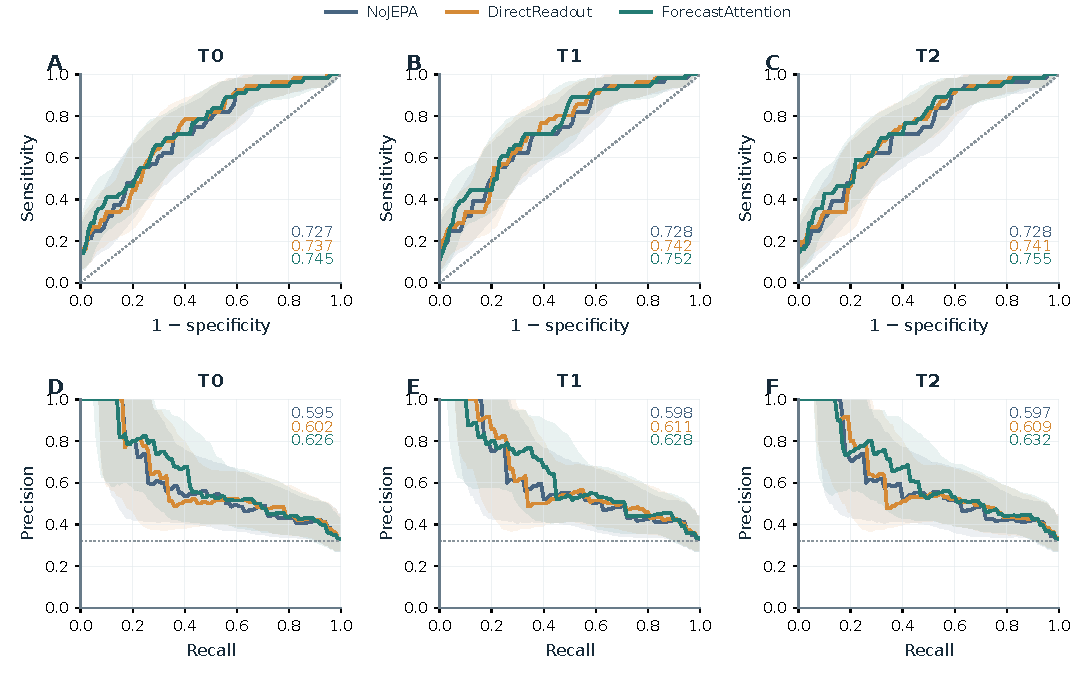
\includegraphics[width=\textwidth]{figures/discrimination.pdf}
\caption{Discrimination of seed-44 five-fold probability ensembles. (A--C) ROC curves; (D--F) precision--recall curves. Each patient's probabilities are averaged across the five fold models before constructing a curve or computing a metric. Shading shows pointwise 95\% paired patient-bootstrap intervals conditional on the fitted ensemble. Colored values give AUROC or non-interpolated AP calculated directly from ensemble scores; grid interpolation may change the plotted area. The dotted PR reference is the 0.32 positive prevalence.}
\label{fig:discrimination}
\end{figure*}

Under direct readout, adding future-state supervision increased macro AUROC by 0.0121, AP by 0.0107, and F1 by 0.0261. The complete forecast-attention readout gave a further AUROC increase of 0.0108 and AP increase of 0.0208, but a F1 decrease of 0.0074 relative to \direct{}. The first comparison more closely isolates auxiliary supervision; the second jointly changes forecast inputs, pooling, and classifier width. The supplementary \meanmodel{} achieved macro AUROC/AP/F1 of 0.7465/0.6139/0.5742 (Table~\ref{tab:pooling}). It therefore had higher F1 than the attention model, despite lower AUROC and AP. Attention did not produce a uniform improvement over mean pooling.

Paired patient intervals qualify these descriptive rankings (Fig.~\ref{fig:paired}). The macro AUROC difference for \fullmodel{} versus \nojepa{} was +0.0228 [0.0012, 0.0465]. The \direct{}--\nojepa{} difference was +0.0121 [$-0.0038$, 0.0287], and the \fullmodel{}--\direct{} difference was +0.0108 [$-0.0101$, 0.0327]. AP and F1 contrasts between the complete model and either direct control had intervals including zero. In particular, the full-versus-direct F1 difference was $-0.0074$ [$-0.0424$, 0.0352]. These intervals condition on a retrospectively selected seed and ensemble policy and exclude their selection uncertainty.

The paired DeLong test for the full-versus-\nojepa{} Macro AUROC difference gave a nominal two-sided $p=0.0462$, increasing to $p_{\mathrm{Holm}}=0.4161$ after adjustment over the nine principal Macro comparisons (Table~\ref{tab:bootstrap}). The corresponding raw/adjusted AUROC values were 0.1401/0.8404 for \direct{} versus \nojepa{} and 0.3055/1.0000 for \fullmodel{} versus \direct{}. None of the nine principal AUROC/AP/F1 comparisons met the adjusted 0.05 criterion. The unadjusted interval excluding zero for the complete-versus-control AUROC therefore does not establish a multiplicity-adjusted difference. These nonsignificant results do not demonstrate equivalence.
\begin{table*}[t]
\centering
\small
\caption{Exploratory principal Macro comparisons. AUROC uses paired DeLong tests with correlated landmark placements averaged per patient. AP and F1 use approximate, null-centered paired patient-bootstrap tests with 99,999 shared resamples. All $p$ values are two-sided. Holm adjustment covers all nine entries in this table. Direct and Attention abbreviate DirectReadout and ForecastAttention. $^{*}p_{\mathrm{Holm}}<0.05$, $^{**}p_{\mathrm{Holm}}<0.01$, $^{***}p_{\mathrm{Holm}}<0.001$; ns, not significant after the stated correction. Intervals are unadjusted 95\% patient-bootstrap intervals (2,000 shared draws) and need not agree with adjusted test decisions. All analyses condition on the fitted, retrospectively selected seed44 ensembles.}
\label{tab:bootstrap}
\begin{tabular}{llrrrc}
\toprule
Comparison & Metric & Difference [95\% CI] & $p$ & $p_{\mathrm{Holm}}$ & Sig. \\
\midrule
Direct -- NoJEPA & AUROC & +0.0121 [-0.0038, +0.0287] & 0.1401 & 0.8404 & ns \\
Direct -- NoJEPA & AP & +0.0107 [-0.0114, +0.0321] & 0.3286 & 1.0000 & ns \\
Direct -- NoJEPA & F1 & +0.0261 [-0.0039, +0.0621] & 0.1150 & 0.8048 & ns \\
Attention -- NoJEPA & AUROC & +0.0228 [+0.0012, +0.0465] & 0.0462 & 0.4161 & ns \\
Attention -- NoJEPA & AP & +0.0315 [-0.0030, +0.0698] & 0.0899 & 0.7190 & ns \\
Attention -- NoJEPA & F1 & +0.0188 [-0.0264, +0.0735] & 0.4471 & 1.0000 & ns \\
Attention -- Direct & AUROC & +0.0108 [-0.0101, +0.0327] & 0.3055 & 1.0000 & ns \\
Attention -- Direct & AP & +0.0208 [-0.0108, +0.0566] & 0.2327 & 1.0000 & ns \\
Attention -- Direct & F1 & -0.0074 [-0.0424, +0.0352] & 0.6995 & 1.0000 & ns \\
\bottomrule
\end{tabular}
\end{table*}


\begin{figure*}[t]
\centering
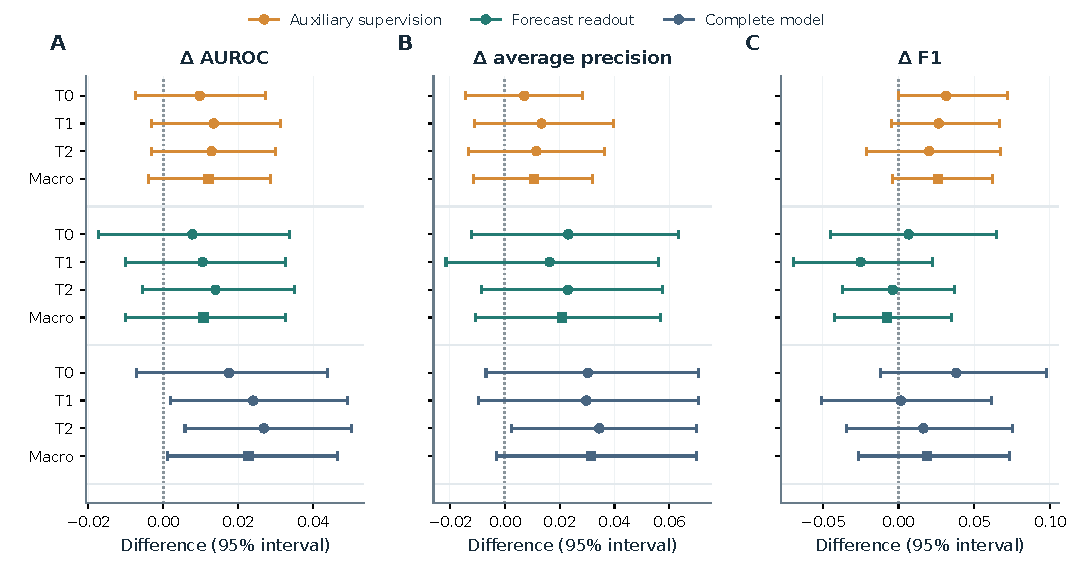
\includegraphics[width=\textwidth]{figures/paired_comparisons.pdf}
\caption{Paired differences between seed-44 ensembles at T0, T1, T2, and the landmark macro. Colors distinguish auxiliary supervision, additional forecast readout, and the complete-model contrast. Squares denote macro estimates. Bars are unadjusted 95\% patient-bootstrap intervals with identical patient draws shared across models and landmarks; adjusted tests are reported separately in Tables~\ref{tab:bootstrap} and~\ref{tab:significance_landmarks}. Five constituent fold models do not represent five independent test cohorts.}
\label{fig:paired}
\end{figure*}

\subsection{Threshold behavior and class imbalance}
\begin{table*}[t]
\centering
\small
\caption{Extended operating-point metrics for seed 44 at probability threshold 0.5. Each patient score is the arithmetic mean of probabilities from the five fold models before any metric is calculated. All landmarks contain the same 175 holdout patients (56 pCR-positive). Macro equally averages the three landmark metric values. PPV and NPV denote positive and negative predictive value; BA is balanced accuracy.}
\label{tab:extended_operating}
\begin{tabular}{llrrrrrr}
\toprule
Model & Stage & Sens. & Spec. & PPV & NPV & BA & MCC \\
\midrule
NoJEPA & T0 & 0.607 & 0.689 & 0.479 & 0.788 & 0.648 & 0.281 \\
NoJEPA & T1 & 0.625 & 0.681 & 0.479 & 0.794 & 0.653 & 0.289 \\
NoJEPA & T2 & 0.625 & 0.689 & 0.486 & 0.796 & 0.657 & 0.298 \\
NoJEPA & Macro & 0.619 & 0.686 & 0.481 & 0.793 & 0.653 & 0.289 \\
\midrule
DirectReadout & T0 & 0.643 & 0.706 & 0.507 & 0.808 & 0.674 & 0.331 \\
DirectReadout & T1 & 0.661 & 0.689 & 0.500 & 0.812 & 0.675 & 0.330 \\
DirectReadout & T2 & 0.679 & 0.664 & 0.487 & 0.814 & 0.671 & 0.321 \\
DirectReadout & Macro & 0.661 & 0.686 & 0.498 & 0.811 & 0.673 & 0.328 \\
\midrule
ForecastAttention & T0 & 0.661 & 0.697 & 0.507 & 0.814 & 0.679 & 0.339 \\
ForecastAttention & T1 & 0.714 & 0.571 & 0.440 & 0.810 & 0.643 & 0.267 \\
ForecastAttention & T2 & 0.714 & 0.613 & 0.465 & 0.820 & 0.664 & 0.306 \\
ForecastAttention & Macro & 0.696 & 0.627 & 0.471 & 0.814 & 0.662 & 0.304 \\
\bottomrule
\end{tabular}
\end{table*}

At threshold 0.5, \fullmodel{} had macro sensitivity 0.6964 and NPV 0.8145, compared with 0.6607 and 0.8113 for \direct{} (Table~\ref{tab:extended_operating}). These increases were accompanied by lower specificity (0.6275 versus 0.6863) and PPV (0.4705 versus 0.4981). The sensitivity difference was +0.0357 [$-0.0106$, 0.1006], while the specificity difference was $-0.0588$ [$-0.0948$, $-0.0234$]. The sensitivity interval therefore included zero even though the specificity decrease was more clearly separated from zero in this conditional analysis.

The full model's operating point varied across landmarks. At T0, it identified 37 positive outcomes and produced 36 false positives. At T1 it identified 40 positive outcomes but produced 51 false positives; at T2 it again identified 40 and produced 46 false positives. Thus the T0--T1 change yielded three additional true positives alongside 15 additional false positives, explaining why improved ranking could coexist with lower F1 at 0.5.

Among the principal models, \direct{} had the highest macro balanced accuracy (0.6735) and MCC (0.3277), compared with 0.6619 and 0.3038 for \fullmodel{} and 0.6527 and 0.2894 for \nojepa{}. Macro raw accuracy was 0.6781, 0.6495, and 0.6648, respectively. All were below the all-negative reference of 0.68 in this cohort. Accuracy alone would therefore obscure discrimination of the minority class. The supplementary \meanmodel{} reached accuracy 0.6838, balanced accuracy 0.6793, and MCC 0.3386.

OOF-selected Youden thresholds changed holdout F1 from 0.5416 to 0.5471 for \nojepa{}, 0.5678 to 0.5713 for \direct{}, and 0.5604 to 0.5631 for \fullmodel{} (Table~\ref{tab:extended_threshold}). For the full model, sensitivity increased to 0.7202 while specificity decreased to 0.6050. In contrast, \meanmodel{} F1 decreased from 0.5742 to 0.5563. These outcomes concern transfer of thresholds fitted on single-model OOF scores to ensemble scores. They neither optimize a holdout threshold nor establish calibration of the ensemble.

\subsection{Longitudinal information and probability quality}
The paired T2--T0 AUROC change was +0.0099 [0.0013, 0.0187] for \fullmodel{}, +0.0006 [$-0.0062$, 0.0070] for \nojepa{}, and +0.0038 [$-0.0064$, 0.0140] for \direct{}. For the full model, the corresponding AP change was +0.0059 [$-0.0098$, 0.0203] and F1 change was $-0.0103$ [$-0.0535$, 0.0340]. Its AUROC improvement therefore did not imply an improvement in every endpoint summary. Outcome-conditioned changes in each patient's ensemble score are shown in Fig.~\ref{fig:scorechanges}.

No comparison met the Holm-adjusted 0.05 criterion in the 81-test secondary family, which includes landmark, operating, probability-quality, pooling, and longitudinal comparisons (Tables~\ref{tab:significance_landmarks}--\ref{tab:significance_longitudinal}). For example, the full model's T2--T0 AUROC change had raw $p=0.0145$ but adjusted $p=1.0000$. The full-versus-direct specificity decrease had raw $p=0.00175$ and adjusted $p=0.14175$. Adjusting all 90 comparisons jointly also yielded no significant result. These tests qualify the descriptive trends without establishing absence of an effect.

\begin{table*}[t]
\centering
\small
\caption{Probability quality of the seed44 fivefold probability ensemble, averaged over T0--T2 metrics. Lower is better. ECE uses ten equal-width bins.}
\label{tab:calibration}
\begin{tabular}{lrrr}
\toprule
Model & NLL & Brier & ECE \\
\midrule
NoJEPA & 0.5822 & 0.2010 & 0.1337 \\
DirectReadout & 0.5819 & 0.2001 & 0.1272 \\
ForecastAttention & 0.5990 & 0.2061 & 0.1687 \\
\bottomrule
\end{tabular}
\end{table*}

Macro NLL/Brier/ECE was 0.5990/0.2061/0.1687 for \fullmodel{}, compared with 0.5819/0.2001/0.1272 for \direct{} and 0.5822/0.2010/0.1337 for \nojepa{}. The complete model's stronger ranking therefore coexisted with worse point estimates of all three probability-quality metrics. Its Brier score and ECE were worse at T1 and T2 than at T0, although AUROC increased across the three visits (Fig.~\ref{fig:longitudinal}). Reliability diagrams provide a complementary description of the ensemble probabilities (Fig.~\ref{fig:calutility}). All 14 macro metrics and their conditional patient intervals are reported in Table~\ref{tab:extended_macro}.

\begin{figure*}[t]
\centering
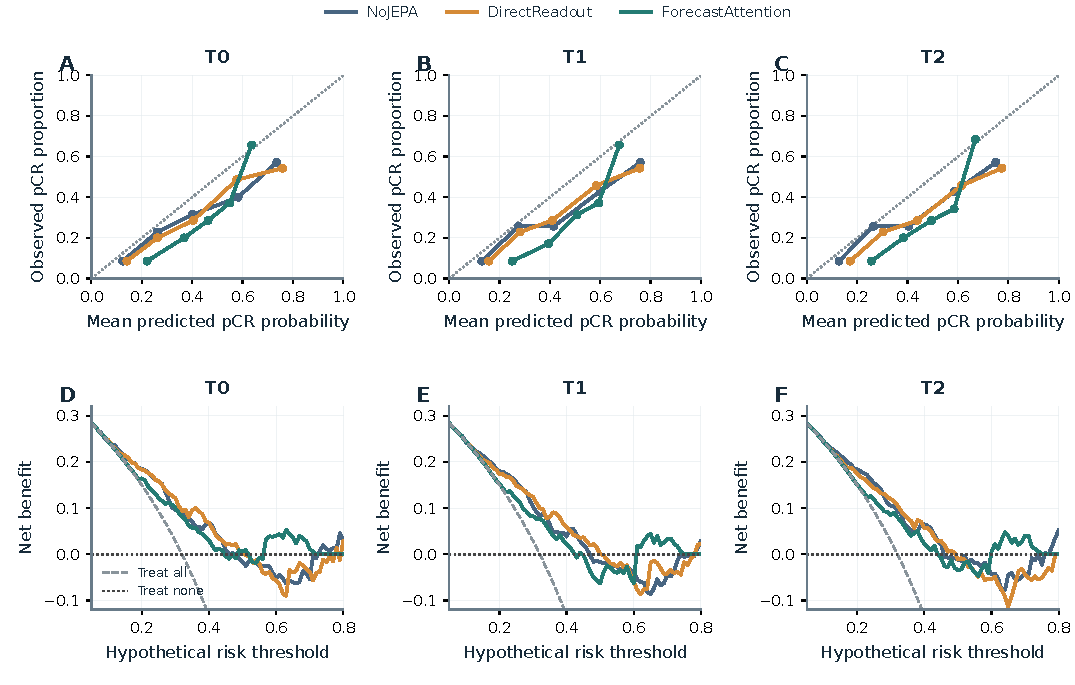
\includegraphics[width=\textwidth]{figures/calibration_utility.pdf}
\caption{Probability quality and hypothetical decision utility of the seed-44 ensembles. (A--C) Reliability diagrams use five equal-count ensemble-probability rank groups, each containing 35 patients; these differ from the ten fixed probability bins used for ECE. (D--F) Net-benefit curves for generic threshold-based positive actions with treat-all and treat-none references. Scores are five-fold mean probabilities without recalibration. No specific escalation or de-escalation strategy is validated.}
\label{fig:calutility}
\end{figure*}

\subsection{Hypothetical net benefit}
Decision curves did not preserve the discrimination ranking across thresholds. At a hypothetical risk threshold of 0.30, macro net benefit was 0.1222 for \direct{} and 0.0890 for \fullmodel{}. At threshold 0.50, all three principal models had negative macro net benefit: $-0.0152$, $-0.0019$, and $-0.0305$ for \nojepa{}, \direct{}, and \fullmodel{}, respectively. At 0.70 the ordering reversed, with +0.0279 for \fullmodel{} and $-0.0413$ for \direct{}. These threshold-dependent values use uncalibrated probabilities and a generic mathematical utility; they do not establish an acceptable clinical operating point.

\subsection{Exploratory biological and acquisition-related subgroups}
All four HR/HER2 groups had positive point estimates of the macro AUROC difference between \fullmodel{} and \nojepa{}, but every corresponding interval included zero (Fig.~\ref{fig:subgroups}; Table~\ref{tab:subgroups}). Differences were +0.0287 [$-0.0318$, 0.0914] in HR-positive/HER2-negative patients (68 patients, 11 positive), +0.0307 [$-0.0750$, 0.1318] in HR-positive/HER2-positive patients (31, 12 positive), +0.0748 [$-0.0251$, 0.2502] in HR-negative/HER2-positive patients (14, 7 positive), and +0.0331 [$-0.0128$, 0.0840] in HR-negative/HER2-negative patients (62, 26 positive). These small exploratory groups do not support a confirmed subtype-specific advantage or interaction.

Operating behavior also differed by group. In HR-positive/HER2-negative patients, the full model's macro sensitivity/specificity was 0.2424/0.9474, compared with 0.0909/0.9825 for \nojepa{}. Improved ranking therefore coexisted with low sensitivity at threshold 0.5. Age and source-namespace analyses are descriptive; the two namespaces belong to the same clinical release and do not constitute external validation. Only 11 patients had partial clipping of the largest predicted baseline component, including one positive outcome. AUROC and AP were suppressed for this group under the minimum-outcome rule.

\begin{figure*}[t]
\centering
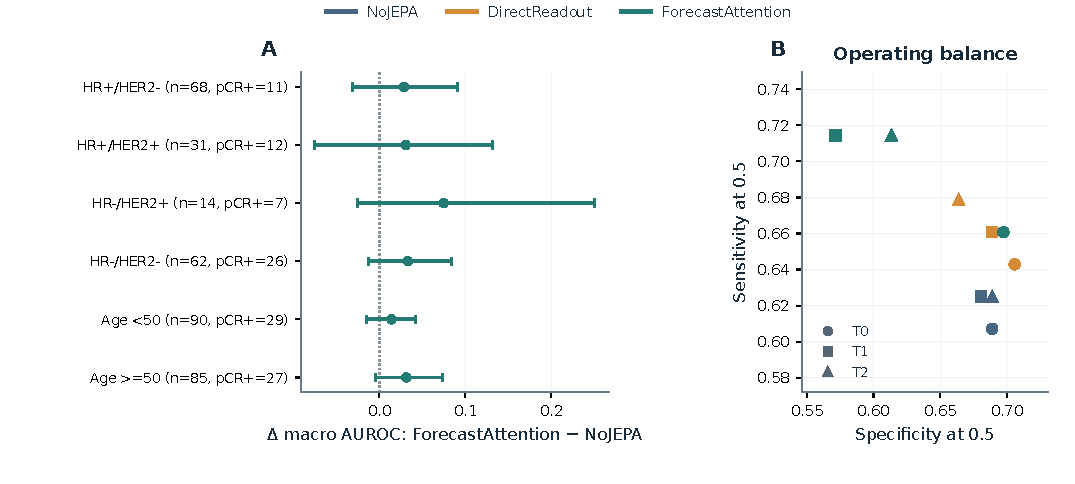
\includegraphics[width=\textwidth]{figures/subgroup_operating.pdf}
\caption{Exploratory subgroup and operating-point summaries from seed-44 ensemble probabilities. (A) Macro AUROC differences between ForecastAttention and NoJEPA within HR/HER2 and age groups, with sample sizes, positive outcomes, and unadjusted paired intervals. No subgroup-interaction claim is made. (B) Specificity and sensitivity at threshold 0.5 across landmarks; colors identify models and markers identify landmarks.}
\label{fig:subgroups}
\end{figure*}

\subsection{Archived forecast and gradient diagnostics}
Archived fixed-training-probe diagnostics provide a separate view of the five individual seed-44 models (Fig.~\ref{fig:mechanism}). At common epoch 20, fold-mean copy-normalized forecast skills for \direct{} were +0.0258, +0.0500, and +0.1935 at one-, two-, and three-step horizons. Corresponding values for \fullmodel{} were $-0.0368$, $-0.0154$, and +0.0242 (Table~\ref{tab:worldprobe}). Each skill is normalized within its own snapshot's EMA coordinates and then averaged across folds; latent states from separate models are not ensembled. The complete model's better pCR ranking cannot simply be attributed to uniformly more accurate latent forecasts under this diagnostic.

The diagnostic requires the real landmark, target, and every intermediate visit, whereas the training objective masks unavailable future targets. Its eligible populations therefore vary by horizon. Only 5--9 patients per training probe were eligible at three steps, and these are not best-checkpoint holdout forecast measurements. The predictor's pCR-loss gradient norm was zero for \direct{} and averaged 0.7148 for \fullmodel{}; weighted rollout-gradient norms were 0.1213 and 0.1308. These values support the expected gradient routing, but gradient magnitude is not a biological effect size. \nojepa{} has no available trained-world diagnostic and is not assigned an artificial zero skill.

\begin{figure*}[t]
\centering
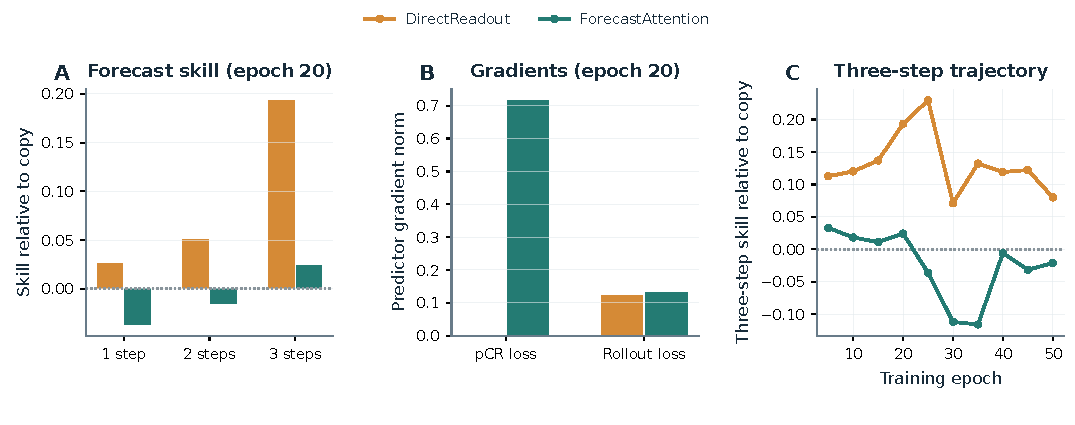
\includegraphics[width=\textwidth]{figures/forecast_mechanism.pdf}
\caption{Archived seed-44 fixed-training-probe diagnostics. (A) Copy-normalized forecast skill at common epoch 20. (B) Predictor gradient norms from pCR and weighted rollout losses. (C) Three-step skill across common archived epochs. Statistics are computed within each model's EMA coordinates and averaged across five folds, distinct from probability ensembling for pCR. These are training diagnostics; real continuous visit chains are required and three-step eligibility is only 5--9 patients per probe.}
\label{fig:mechanism}
\end{figure*}

\section{Discussion}
\label{sec:discussion}
\subsection{Distinguishing supervision, forecast readout, and forecasting fidelity}
The seed-44 probability ensembles support a descriptive hierarchy in macro AUROC and AP: auxiliary supervision improves the direct-readout point estimates, and the complete forecast-attention readout improves them further. Only the complete-versus-NoJEPA macro AUROC interval excludes zero among these principal AUROC contrasts, but its nominal DeLong $p=0.0462$ becomes 0.4161 after Holm adjustment. None of the nine principal comparisons meets the adjusted criterion. Moreover, direct readout has higher macro F1 than forecast attention, and the mean-pooling control has the highest macro F1 among all four models. The ranking differences remain exploratory point-estimate advantages under this selected policy; they do not establish superiority or that attention is necessary.

The archived probes also challenge an explanation based solely on more accurate future states. At common epoch 20, the auxiliary-supervised direct models have better copy-normalized latent forecast skill than the full models, while the full probability ensemble has better pCR ranking. A possible explanation is that classification gradients shape forecast features toward endpoint-relevant directions at the expense of some fidelity to the EMA target. The nonzero pCR-to-predictor gradient is consistent with this pathway. However, fold-averaged training diagnostics in separately learned spaces cannot establish that mechanism or demonstrate anatomical forecasting quality. They are evaluated at a different level from the ensemble pCR predictor.

Useful future controls include classifier-width-matched direct readout, stopped-gradient forecast features, copy-state readout, and independent holdout forecast evaluation. The main models predict embeddings rather than generate MRI for classification. The internal name \nojepa{} denotes removal of the future-state objective while retaining shared fusion and transition queries. The forecast-versus-direct comparison also changes classifier width and feature groups, so it cannot isolate attention alone.

\subsection{What additional visits change}
The complete ensemble's AUROC increases across T0--T2 on the same patients, with a paired T2--T0 difference of +0.0099. Its F1 is nevertheless lower at T2 than at T0 and falls most at T1. The increased number of positive predictions identifies additional true positives but also adds false positives. These error counts explain why later information and improved ranking need not improve a fixed-threshold decision rule. Outcome-conditioned probability-change histograms describe ensemble score movement; they do not establish that every patient's prediction becomes more accurate.

T0 imaging preceded randomization, while the model is conditioned on the eventual assigned arm. This remains a retrospective conditional scenario. The arm encoding does not capture delivered dose, cycle timing, dose reductions, adherence, or treatment changes. Altering the arm token cannot identify an individual treatment effect without suitable causal assumptions and exposure data. Complete T0--T2 holdout eligibility also restricts the population to which the longitudinal comparison applies.

\subsection{Classification, calibration, and hypothetical utility}
The additional metrics reveal differences hidden by AUROC alone. Compared with direct readout, the complete model has higher point estimates of macro sensitivity and NPV but lower specificity, PPV, balanced accuracy, MCC, and F1. The sensitivity-difference interval includes zero, while the specificity-difference interval excludes zero conditionally on these fitted models. The latter is an unadjusted interval: its paired bootstrap test does not meet the secondary-family Holm criterion ($p_{\mathrm{Holm}}=0.14175$). All three principal models have macro raw accuracy below the all-negative reference of 0.68, although their AUROCs exceed 0.72. Raw accuracy would therefore obscure detection of the minority positive class.

The full model's NLL, Brier score, and ECE are also worse than the direct controls' point estimates. Probability ensembling does not by itself establish calibration. The OOF Youden analysis changes operating points, with small F1 increases for the principal models but a decrease for mean pooling. OOF development scores originate from one held-out fold model per patient, whereas holdout scores average five models. Transferring a threshold between these score distributions is a sensitivity analysis; it cannot replace independent ensemble calibration or validation of a clinical threshold.

Net-benefit rankings change with the hypothetical threshold. Direct readout has higher macro net benefit at 0.30, while forecast attention has higher net benefit at 0.70; all principal variants have negative macro values at 0.50. These are summaries under a generic positive-action utility, not evaluations of a defined care pathway. A clinically motivated operating point would require the consequences of false-positive and false-negative actions to be specified and calibration to be fitted without holdout leakage.

\subsection{Subgroup inference and transportability}
The four HR/HER2 groups have positive full-versus-control macro AUROC differences, but all paired intervals include zero. Their magnitudes differ and the smallest group has only 14 patients. These summaries provide no confirmed subgroup interaction or subtype-specific benefit. In HR-positive/HER2-negative patients, low sensitivity at 0.5 persists despite improved ranking; the group's low prevalence informs predictive values but does not itself explain sensitivity.

Source namespaces share one clinical release and do not supply independent external validation. Crop sensitivity analysis is similarly constrained: the 11 patients with partial clipping contain only one positive outcome, preventing reliable discrimination assessment under the stated minimum-outcome rule. Reporting the denominator and suppressing AUROC/AP is more informative than interpreting an unstable point estimate.

\subsection{Limitations and a confirmatory study}
\label{sec:limitations}
Seed 44 and probability ensembling were selected after holdout results were available. Patient bootstrap intervals condition on these fitted ensembles and fixed OOF thresholds. They exclude retraining, seed choice, aggregation choice, model selection, and threshold-selection uncertainty, and remain unadjusted for multiple comparisons. Separate Holm adjustments for the nine principal and 81 secondary tests, with an additional all-90 sensitivity analysis, do not remove retrospective selection bias. The testing methods and reporting families were also chosen retrospectively. DeLong inference is asymptotic, and null-centered bootstrap tests are approximate; finite-sample behavior can be problematic for non-smooth metrics such as AP, F1, and binned ECE. Neither adjusted family yielded a significant result, and nonsignificance does not demonstrate equivalence. One selected seed does not establish training stability. The reported predictor requires five fold models at inference, and its performance should not be interpreted as that of one model trained on the full development cohort. A confirmatory analysis should lock training, aggregation, and statistical policies before evaluating independent patients.

The holdout is an internal downstream split. Twenty-nine of its patients had belonged to an earlier development split. Current supervised models were retrained using the new patient-disjoint folds and were not warm-started from those earlier pCR models, but codec and localization-model pretraining have not been fully audited for current-holdout overlap. This prevents a claim that every pipeline stage was evaluated on wholly unseen patients.

Fixed baseline localization and cropping may omit multifocal disease or changes outside the field of view. Geometry and array checks do not establish anatomical registration accuracy. Holdout patients have complete T0--T2 imaging, whereas development retains incomplete histories; missingness, acquisition variation, and subtype prevalence may limit transportability. Archived training probes do not replace best-checkpoint holdout forecast evaluation and have small long-horizon denominators.

The study remains an internal architectural comparison. Matched clinical-only, conventional imaging, and independent longitudinal baselines are still needed, along with external validation, anatomical quality review, and independently assessed calibration. Precise pCR pathology criteria, scan intervals, ethics determination, and upstream provenance also require final documentation before submission.

\section{Conclusion}
Using seed 44 and patient-wise mean probabilities from five fold models, forecast-attention readout achieved the highest AUROC and AP among the principal variants. Direct readout had higher macro F1, while the supplementary mean-pooling model had the highest macro F1 among all four models. None of the nine principal comparisons or 81 secondary comparisons met its Holm-adjusted significance criterion. Expanded evaluation revealed descriptive differences in specificity, calibration, subgroup uncertainty, and threshold-dependent net benefit, and training probes did not support attributing improved ranking simply to more accurate latent forecasts. These exploratory results motivate independent validation, complete upstream provenance, stronger matched baselines, and prospectively fixed seed, ensembling, statistical, and operating-point policies.

\section*{Data and code availability}
Source imaging collections are available through The Cancer Imaging Archive, subject to their applicable access conditions and licenses. The present derived manifests, processing lineage, and evaluation outputs are retained locally. \todo{Specify the public repository, versioned release, permitted derived-data artifacts, and access mechanism before submission; no public code-release claim is made in this draft.}
\section*{Ethics approval and consent}
\todo{Provide the original studies' ethics and consent statements and the local institutional determination for this secondary analysis, including an approval or exemption identifier where applicable. Public availability alone is not an ethics approval.}
\section*{Funding}
\todo{Provide grant numbers and the funders' roles, or confirm that no specific funding was received.}
\section*{Declaration of competing interest}
\todo{Obtain and insert the actual declarations from every author.}
\section*{CRediT authorship contribution statement}
\todo{Provide author names and agreed contributions; no authorship or contributions have been inferred.}
\section*{Declaration of generative AI and AI-assisted technologies in the manuscript preparation process}
During preparation of this initial draft, OpenAI Codex was used to organize source evidence, generate reproducible aggregate tables and figures, and assist with English drafting. \todo{All authors must review and edit the manuscript, verify every statement and reference, and finalize the disclosure under the journal's current policy before submission.}
\clearpage
\appendix
\section{Supplementary pooling, metrics, and uncertainty}
\label{sec:supplement}
The supplementary \meanmodel{} uses the same training seed 44, five-fold probability-ensemble rule, observed-history protocol, future-state objective, and forecast classifier feature groups as \fullmodel{}, replacing spatial attention with mean pooling. Its metrics are computed from patient-wise mean probabilities, consistent with the main analysis.
\begin{table*}[t]
\centering
\small
\caption{Supplementary pooling comparison using seed44 fivefold probability ensembles. ForecastMean and ForecastAttention share forecast readout and future-state supervision, differing in spatial pooling. Probabilities are averaged before metrics; Macro averages the three landmarks.}
\label{tab:pooling}
\begin{tabular}{llrrr}
\toprule
Model & Landmark & AUROC & AP & F1 \\
\midrule
ForecastMean & T0 & 0.7431 & 0.6088 & 0.5625 \\
ForecastMean & T1 & 0.7494 & 0.6121 & 0.5865 \\
ForecastMean & T2 & 0.7471 & 0.6209 & 0.5736 \\
ForecastMean & Macro & 0.7465 & 0.6139 & 0.5742 \\
ForecastAttention & T0 & 0.7450 & 0.6256 & 0.5736 \\
ForecastAttention & T1 & 0.7521 & 0.6278 & 0.5442 \\
ForecastAttention & T2 & 0.7550 & 0.6315 & 0.5634 \\
ForecastAttention & Macro & 0.7507 & 0.6283 & 0.5604 \\
\bottomrule
\end{tabular}
\end{table*}

\begin{table*}[t]
\centering
\footnotesize
\setlength{\tabcolsep}{5pt}
\caption{All 14 macro metrics for the principal variants: point estimate [95\% patient-bootstrap percentile interval]. Each patient\textquotesingle s five seed44 fold-model probabilities are averaged first; metrics are then computed and equally averaged over T0--T2. Threshold-dependent metrics use 0.5. Identical patient resamples preserve pairing across models and landmarks. Entries are marginal model intervals; paired differences are reported separately. Intervals condition on the fitted ensembles and exclude retraining and retrospective selection uncertainty. Downward arrows identify metrics for which lower is better.}
\label{tab:extended_macro}
\begin{tabular}{lccc}
\toprule
Metric & NoJEPA & DirectReadout & ForecastAttention \\
\midrule
AUROC & 0.7279 [0.6501, 0.8046] & 0.7399 [0.6653, 0.8155] & 0.7507 [0.6741, 0.8268] \\
AP & 0.5968 [0.4703, 0.7141] & 0.6075 [0.4816, 0.7235] & 0.6283 [0.5066, 0.7465] \\
F1 & 0.5416 [0.4330, 0.6397] & 0.5678 [0.4626, 0.6612] & 0.5604 [0.4605, 0.6564] \\
Accuracy & 0.6648 [0.5980, 0.7334] & 0.6781 [0.6114, 0.7429] & 0.6495 [0.5829, 0.7181] \\
Sensitivity & 0.6190 [0.4909, 0.7487] & 0.6607 [0.5333, 0.7836] & 0.6964 [0.5723, 0.8187] \\
Specificity & 0.6863 [0.6043, 0.7667] & 0.6863 [0.6048, 0.7634] & 0.6275 [0.5478, 0.7057] \\
PPV & 0.4815 [0.3667, 0.5970] & 0.4981 [0.3892, 0.6117] & 0.4705 [0.3684, 0.5774] \\
NPV & 0.7929 [0.7130, 0.8695] & 0.8113 [0.7352, 0.8865] & 0.8145 [0.7347, 0.8917] \\
Balanced accuracy & 0.6527 [0.5759, 0.7268] & 0.6735 [0.6016, 0.7460] & 0.6619 [0.5930, 0.7360] \\
MCC & 0.2894 [0.1454, 0.4312] & 0.3277 [0.1906, 0.4617] & 0.3038 [0.1737, 0.4424] \\
Youden index & 0.3053 [0.1518, 0.4535] & 0.3470 [0.2031, 0.4919] & 0.3239 [0.1861, 0.4720] \\
NLL $\downarrow$ & 0.5822 [0.5192, 0.6442] & 0.5819 [0.5213, 0.6418] & 0.5990 [0.5613, 0.6364] \\
Brier score $\downarrow$ & 0.2010 [0.1739, 0.2279] & 0.2001 [0.1735, 0.2268] & 0.2061 [0.1883, 0.2235] \\
ECE $\downarrow$ & 0.1337 [0.0979, 0.2015] & 0.1272 [0.0901, 0.1964] & 0.1687 [0.1175, 0.2281] \\
\bottomrule
\end{tabular}
\end{table*}

\begin{table*}[t]
\centering
\small
\caption{Operating-point sensitivity analysis for seed-44 test ensemble scores, shown as three-landmark metric means. The alternative threshold maximizes Youden index on concatenated, disjoint out-of-fold development predictions, separately at each landmark; the largest threshold breaks ties. Each development patient contributes one score from a model that did not train on that patient. OOF scores arise from single fold models, whereas test scores average five model probabilities: this distribution mismatch makes this a sensitivity analysis, not validated ensemble calibration. No test labels select thresholds.}
\label{tab:extended_threshold}
\begin{tabular}{llrrrr}
\toprule
Model & Policy & F1 & Sens. & Spec. & MCC \\
\midrule
NoJEPA & 0.5 & 0.542 & 0.619 & 0.686 & 0.289 \\
NoJEPA & OOF validation Youden & 0.547 & 0.655 & 0.653 & 0.289 \\
\midrule
DirectReadout & 0.5 & 0.568 & 0.661 & 0.686 & 0.328 \\
DirectReadout & OOF validation Youden & 0.571 & 0.655 & 0.700 & 0.336 \\
\midrule
ForecastAttention & 0.5 & 0.560 & 0.696 & 0.627 & 0.304 \\
ForecastAttention & OOF validation Youden & 0.563 & 0.720 & 0.605 & 0.304 \\
\bottomrule
\end{tabular}
\end{table*}


\subsection{Paired significance checks}
Table~\ref{tab:bootstrap} combines the principal Macro comparisons with their unadjusted 95\% patient-bootstrap intervals, raw two-sided $p$ values, and Holm-adjusted $p$ values for the nine-test principal family. AUROC uses paired DeLong tests; other metrics use approximate null-centered paired patient-bootstrap tests with 99,999 shared patient resamples. The secondary family comprises 81 tests, reported in Tables~\ref{tab:significance_landmarks}--\ref{tab:significance_longitudinal}. These use the same seed-44 ensemble predictions and the same 175 patients, retaining model and landmark dependence. A significance marker refers to its stated Holm-adjusted family; ns denotes $p_{\mathrm{Holm}}\geq0.05$. The existing unadjusted 2,000-resample percentile intervals are not exact inversions of these tests and do not establish significance after correction. The original score-swap tests are retained separately in the source package: they test the stronger score-exchangeability null and do not determine these markers. The main testing method was revised after inspecting initial score-swap results; all tests and reporting choices remain retrospective and exploratory.

\begin{table*}[t]
\centering
\small
\caption{Exploratory landmark comparisons. AUROC uses paired DeLong tests; other metrics use approximate, null-centered paired patient-bootstrap tests (99,999 shared resamples). All $p$ values are two-sided. $p_{\mathrm{Holm}}$ adjusts jointly over the 81 secondary tests in Tables~\ref{tab:significance_landmarks}--\ref{tab:significance_longitudinal}. Direct and Attention abbreviate DirectReadout and ForecastAttention. $^{*}p_{\mathrm{Holm}}<0.05$, $^{**}p_{\mathrm{Holm}}<0.01$, $^{***}p_{\mathrm{Holm}}<0.001$; ns, not significant after the stated correction. Intervals are unadjusted 95\% patient-bootstrap intervals (2,000 shared draws) and need not agree with adjusted test decisions. All analyses condition on the fitted, retrospectively selected seed44 ensembles.}
\label{tab:significance_landmarks}
\begin{tabular}{lllrrrc}
\toprule
Comparison & Landmark & Metric & Difference [95\% CI] & $p$ & $p_{\mathrm{Holm}}$ & Sig. \\
\midrule
Direct -- NoJEPA & T0 & AUROC & +0.0098 [-0.0074, +0.0274] & 0.2414 & 1.0000 & ns \\
Direct -- NoJEPA & T0 & AP & +0.0071 [-0.0144, +0.0283] & 0.4821 & 1.0000 & ns \\
Direct -- NoJEPA & T0 & F1 & +0.0315 [+0.0000, +0.0722] & 0.0886 & 1.0000 & ns \\
Direct -- NoJEPA & T1 & AUROC & +0.0135 [-0.0032, +0.0312] & 0.1218 & 1.0000 & ns \\
Direct -- NoJEPA & T1 & AP & +0.0134 [-0.0111, +0.0397] & 0.2842 & 1.0000 & ns \\
Direct -- NoJEPA & T1 & F1 & +0.0266 [-0.0047, +0.0669] & 0.1543 & 1.0000 & ns \\
Direct -- NoJEPA & T2 & AUROC & +0.0129 [-0.0032, +0.0299] & 0.1233 & 1.0000 & ns \\
Direct -- NoJEPA & T2 & AP & +0.0115 [-0.0133, +0.0365] & 0.3588 & 1.0000 & ns \\
Direct -- NoJEPA & T2 & F1 & +0.0203 [-0.0209, +0.0671] & 0.3585 & 1.0000 & ns \\
Attention -- NoJEPA & T0 & AUROC & +0.0176 [-0.0071, +0.0439] & 0.1598 & 1.0000 & ns \\
Attention -- NoJEPA & T0 & AP & +0.0303 [-0.0068, +0.0705] & 0.1305 & 1.0000 & ns \\
Attention -- NoJEPA & T0 & F1 & +0.0382 [-0.0119, +0.0974] & 0.1802 & 1.0000 & ns \\
Attention -- NoJEPA & T1 & AUROC & +0.0240 [+0.0019, +0.0492] & 0.0424 & 1.0000 & ns \\
Attention -- NoJEPA & T1 & AP & +0.0297 [-0.0094, +0.0707] & 0.1462 & 1.0000 & ns \\
Attention -- NoJEPA & T1 & F1 & +0.0016 [-0.0506, +0.0616] & 0.9564 & 1.0000 & ns \\
Attention -- NoJEPA & T2 & AUROC & +0.0269 [+0.0058, +0.0502] & 0.0150 & 1.0000 & ns \\
Attention -- NoJEPA & T2 & AP & +0.0345 [+0.0025, +0.0700] & 0.0450 & 1.0000 & ns \\
Attention -- NoJEPA & T2 & F1 & +0.0165 [-0.0343, +0.0756] & 0.5574 & 1.0000 & ns \\
Attention -- Direct & T0 & AUROC & +0.0078 [-0.0172, +0.0337] & 0.5342 & 1.0000 & ns \\
Attention -- Direct & T0 & AP & +0.0231 [-0.0123, +0.0634] & 0.2375 & 1.0000 & ns \\
Attention -- Direct & T0 & F1 & +0.0067 [-0.0450, +0.0650] & 0.8132 & 1.0000 & ns \\
Attention -- Direct & T1 & AUROC & +0.0105 [-0.0101, +0.0326] & 0.3113 & 1.0000 & ns \\
Attention -- Direct & T1 & AP & +0.0163 [-0.0214, +0.0561] & 0.3968 & 1.0000 & ns \\
Attention -- Direct & T1 & F1 & -0.0250 [-0.0693, +0.0225] & 0.2870 & 1.0000 & ns \\
Attention -- Direct & T2 & AUROC & +0.0140 [-0.0056, +0.0350] & 0.1612 & 1.0000 & ns \\
Attention -- Direct & T2 & AP & +0.0230 [-0.0084, +0.0575] & 0.1754 & 1.0000 & ns \\
Attention -- Direct & T2 & F1 & -0.0038 [-0.0372, +0.0370] & 0.8416 & 1.0000 & ns \\
\bottomrule
\end{tabular}
\end{table*}

\begin{table*}[t]
\centering
\small
\caption{Exploratory Macro operating and probability-quality comparisons. Differences are first-named minus second-named model; negative Brier, NLL, or ECE differences favor the first model. AUROC uses paired DeLong tests; other metrics use approximate, null-centered paired patient-bootstrap tests (99,999 shared resamples). All $p$ values are two-sided. $p_{\mathrm{Holm}}$ adjusts jointly over the 81 secondary tests in Tables~\ref{tab:significance_landmarks}--\ref{tab:significance_longitudinal}. Direct and Attention abbreviate DirectReadout and ForecastAttention. $^{*}p_{\mathrm{Holm}}<0.05$, $^{**}p_{\mathrm{Holm}}<0.01$, $^{***}p_{\mathrm{Holm}}<0.001$; ns, not significant after the stated correction. Intervals are unadjusted 95\% patient-bootstrap intervals (2,000 shared draws) and need not agree with adjusted test decisions. All analyses condition on the fitted, retrospectively selected seed44 ensembles.}
\label{tab:significance_extended}
\begin{tabular}{llrrrc}
\toprule
Comparison & Metric & Difference [95\% CI] & $p$ & $p_{\mathrm{Holm}}$ & Sig. \\
\midrule
Direct -- NoJEPA & Accuracy & +0.0133 [-0.0133, +0.0419] & 0.3670 & 1.0000 & ns \\
Direct -- NoJEPA & Sensitivity & +0.0417 [+0.0053, +0.0920] & 0.0652 & 1.0000 & ns \\
Direct -- NoJEPA & Specificity & +0.0000 [-0.0347, +0.0361] & 1.0000 & 1.0000 & ns \\
Direct -- NoJEPA & PPV & +0.0166 [-0.0159, +0.0501] & 0.3087 & 1.0000 & ns \\
Direct -- NoJEPA & NPV & +0.0184 [-0.0002, +0.0429] & 0.0844 & 1.0000 & ns \\
Direct -- NoJEPA & Balanced accuracy & +0.0208 [-0.0046, +0.0513] & 0.1401 & 1.0000 & ns \\
Direct -- NoJEPA & MCC & +0.0382 [-0.0108, +0.0949] & 0.1548 & 1.0000 & ns \\
Direct -- NoJEPA & Youden index & +0.0417 [-0.0092, +0.1025] & 0.1401 & 1.0000 & ns \\
Direct -- NoJEPA & Brier & -0.0010 [-0.0064, +0.0045] & 0.7351 & 1.0000 & ns \\
Direct -- NoJEPA & NLL & -0.0002 [-0.0132, +0.0123] & 0.9753 & 1.0000 & ns \\
Direct -- NoJEPA & ECE & -0.0064 [-0.0460, +0.0224] & 0.6965 & 1.0000 & ns \\
Attention -- NoJEPA & Accuracy & -0.0152 [-0.0533, +0.0248] & 0.4706 & 1.0000 & ns \\
Attention -- NoJEPA & Sensitivity & +0.0774 [+0.0161, +0.1533] & 0.0278 & 1.0000 & ns \\
Attention -- NoJEPA & Specificity & -0.0588 [-0.1053, -0.0122] & 0.0126 & 1.0000 & ns \\
Attention -- NoJEPA & PPV & -0.0110 [-0.0560, +0.0352] & 0.6200 & 1.0000 & ns \\
Attention -- NoJEPA & NPV & +0.0216 [-0.0084, +0.0596] & 0.2119 & 1.0000 & ns \\
Attention -- NoJEPA & Balanced accuracy & +0.0093 [-0.0289, +0.0535] & 0.6568 & 1.0000 & ns \\
Attention -- NoJEPA & MCC & +0.0144 [-0.0580, +0.0989] & 0.7140 & 1.0000 & ns \\
Attention -- NoJEPA & Youden index & +0.0186 [-0.0579, +0.1070] & 0.6568 & 1.0000 & ns \\
Attention -- NoJEPA & Brier & +0.0050 [-0.0072, +0.0173] & 0.4361 & 1.0000 & ns \\
Attention -- NoJEPA & NLL & +0.0169 [-0.0128, +0.0469] & 0.2842 & 1.0000 & ns \\
Attention -- NoJEPA & ECE & +0.0350 [-0.0220, +0.0582] & 0.1477 & 1.0000 & ns \\
Attention -- Direct & Accuracy & -0.0286 [-0.0590, +0.0038] & 0.0733 & 1.0000 & ns \\
Attention -- Direct & Sensitivity & +0.0357 [-0.0106, +0.1006] & 0.2156 & 1.0000 & ns \\
Attention -- Direct & Specificity & -0.0588 [-0.0948, -0.0234] & 0.0018 & 0.1418 & ns \\
Attention -- Direct & PPV & -0.0276 [-0.0611, +0.0076] & 0.1070 & 1.0000 & ns \\
Attention -- Direct & NPV & +0.0032 [-0.0207, +0.0356] & 0.8181 & 1.0000 & ns \\
Attention -- Direct & Balanced accuracy & -0.0116 [-0.0424, +0.0251] & 0.4824 & 1.0000 & ns \\
Attention -- Direct & MCC & -0.0238 [-0.0811, +0.0458] & 0.4360 & 1.0000 & ns \\
Attention -- Direct & Youden index & -0.0231 [-0.0848, +0.0502] & 0.4824 & 1.0000 & ns \\
Attention -- Direct & Brier & +0.0060 [-0.0056, +0.0177] & 0.3135 & 1.0000 & ns \\
Attention -- Direct & NLL & +0.0171 [-0.0103, +0.0444] & 0.2285 & 1.0000 & ns \\
Attention -- Direct & ECE & +0.0415 [-0.0072, +0.0570] & 0.0440 & 1.0000 & ns \\
\bottomrule
\end{tabular}
\end{table*}

\begin{table*}[t]
\centering
\small
\caption{Exploratory pooling comparisons: ForecastAttention minus ForecastMean. AUROC uses paired DeLong tests; other metrics use approximate, null-centered paired patient-bootstrap tests (99,999 shared resamples). All $p$ values are two-sided. $p_{\mathrm{Holm}}$ adjusts jointly over the 81 secondary tests in Tables~\ref{tab:significance_landmarks}--\ref{tab:significance_longitudinal}. Direct and Attention abbreviate DirectReadout and ForecastAttention. $^{*}p_{\mathrm{Holm}}<0.05$, $^{**}p_{\mathrm{Holm}}<0.01$, $^{***}p_{\mathrm{Holm}}<0.001$; ns, not significant after the stated correction. Intervals are unadjusted 95\% patient-bootstrap intervals (2,000 shared draws) and need not agree with adjusted test decisions. All analyses condition on the fitted, retrospectively selected seed44 ensembles.}
\label{tab:significance_pooling}
\begin{tabular}{llrrrc}
\toprule
Landmark & Metric & Difference [95\% CI] & $p$ & $p_{\mathrm{Holm}}$ & Sig. \\
\midrule
T0 & AUROC & +0.0020 [-0.0177, +0.0227] & 0.8443 & 1.0000 & ns \\
T0 & AP & +0.0169 [-0.0182, +0.0548] & 0.3487 & 1.0000 & ns \\
T0 & F1 & +0.0111 [-0.0300, +0.0575] & 0.6113 & 1.0000 & ns \\
T1 & AUROC & +0.0027 [-0.0176, +0.0230] & 0.7866 & 1.0000 & ns \\
T1 & AP & +0.0157 [-0.0211, +0.0518] & 0.3935 & 1.0000 & ns \\
T1 & F1 & -0.0422 [-0.0771, -0.0059] & 0.0203 & 1.0000 & ns \\
T2 & AUROC & +0.0078 [-0.0116, +0.0296] & 0.4393 & 1.0000 & ns \\
T2 & AP & +0.0106 [-0.0224, +0.0438] & 0.5218 & 1.0000 & ns \\
T2 & F1 & -0.0103 [-0.0533, +0.0406] & 0.6604 & 1.0000 & ns \\
Macro & AUROC & +0.0042 [-0.0140, +0.0240] & 0.6626 & 1.0000 & ns \\
Macro & AP & +0.0144 [-0.0190, +0.0476] & 0.3891 & 1.0000 & ns \\
Macro & F1 & -0.0138 [-0.0460, +0.0233] & 0.4174 & 1.0000 & ns \\
\bottomrule
\end{tabular}
\end{table*}

\begin{table*}[t]
\centering
\small
\caption{Exploratory paired T2 minus T0 comparisons. DeLong placements and bootstrap draws retain within-patient dependence between landmarks. AUROC uses paired DeLong tests; other metrics use approximate, null-centered paired patient-bootstrap tests (99,999 shared resamples). All $p$ values are two-sided. $p_{\mathrm{Holm}}$ adjusts jointly over the 81 secondary tests in Tables~\ref{tab:significance_landmarks}--\ref{tab:significance_longitudinal}. Direct and Attention abbreviate DirectReadout and ForecastAttention. $^{*}p_{\mathrm{Holm}}<0.05$, $^{**}p_{\mathrm{Holm}}<0.01$, $^{***}p_{\mathrm{Holm}}<0.001$; ns, not significant after the stated correction. Intervals are unadjusted 95\% patient-bootstrap intervals (2,000 shared draws) and need not agree with adjusted test decisions. All analyses condition on the fitted, retrospectively selected seed44 ensembles.}
\label{tab:significance_longitudinal}
\begin{tabular}{llrrrc}
\toprule
Model & Metric & Difference [95\% CI] & $p$ & $p_{\mathrm{Holm}}$ & Sig. \\
\midrule
NoJEPA & AUROC & +0.0006 [-0.0062, +0.0070] & 0.8441 & 1.0000 & ns \\
NoJEPA & AP & +0.0017 [-0.0100, +0.0125] & 0.7254 & 1.0000 & ns \\
NoJEPA & F1 & +0.0114 [+0.0000, +0.0396] & 0.5334 & 1.0000 & ns \\
DirectReadout & AUROC & +0.0038 [-0.0064, +0.0140] & 0.4384 & 1.0000 & ns \\
DirectReadout & AP & +0.0061 [-0.0109, +0.0248] & 0.4881 & 1.0000 & ns \\
DirectReadout & F1 & +0.0002 [-0.0336, +0.0395] & 0.9922 & 1.0000 & ns \\
ForecastAttention & AUROC & +0.0099 [+0.0013, +0.0187] & 0.0145 & 1.0000 & ns \\
ForecastAttention & AP & +0.0059 [-0.0098, +0.0203] & 0.4225 & 1.0000 & ns \\
ForecastAttention & F1 & -0.0103 [-0.0535, +0.0340] & 0.6492 & 1.0000 & ns \\
\bottomrule
\end{tabular}
\end{table*}


\begin{figure*}[t]
\centering
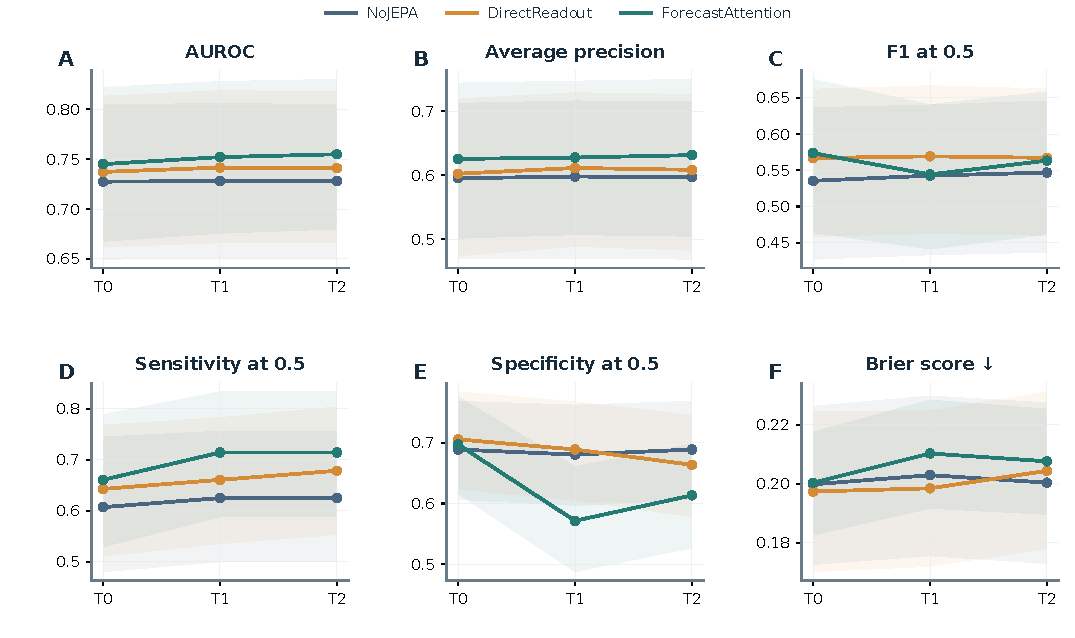
\includegraphics[width=\textwidth]{figures/landmark_performance.pdf}
\caption{Six complementary landmark summaries: AUROC, AP, F1, sensitivity, specificity, and Brier score. All points are calculated from the seed-44 five-fold ensemble probabilities; shading is the conditional 95\% patient-bootstrap interval. The same 175 patients appear at every landmark. A trend in ranking can coexist with a different trend in calibration or error types.}
\label{fig:longitudinal}
\end{figure*}

\begin{figure*}[t]
\centering
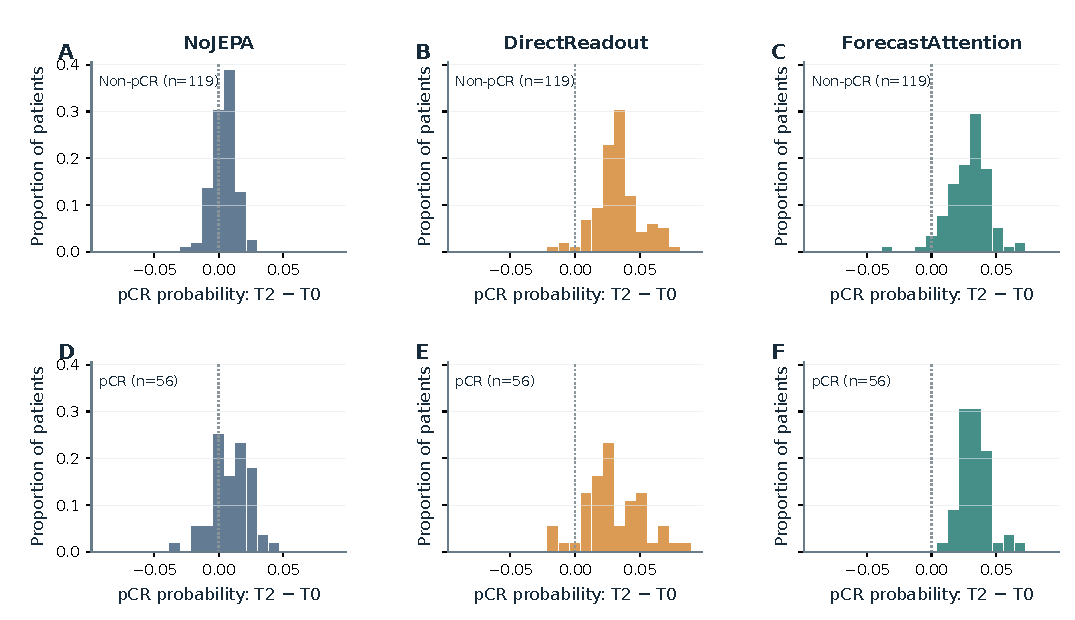
\includegraphics[width=\textwidth]{figures/outcome_score_changes.pdf}
\caption{Outcome-conditioned changes in predicted pCR probability from T0 to T2. Panels separate models and outcome classes. Histograms are calculated directly from the seed-44 five-fold ensemble probability changes for each patient. Changes describe model scores and do not establish an individual treatment effect.}
\label{fig:scorechanges}
\end{figure*}

\section{Supplementary subgroup and training-probe summaries}
\begin{table*}[t]
\centering
\small
\caption{Exploratory subgroup discrimination for the seed44 fivefold probability ensemble. Each patient\textquotesingle s probabilities are averaged over five fold models before computing AUROC; Macro then averages T0--T2 AUROCs. Intervals are paired patient-bootstrap intervals for ForecastAttention minus NoJEPA, conditional on the fitted ensemble. Age 50 is an exploratory reporting cutpoint. Namespace groups are parts of one clinical release, not external cohorts.}
\label{tab:subgroups}
\begin{tabular}{lrrr}
\toprule
Subgroup ($n$/pCR+) & NoJEPA & Full & $\Delta$ AUROC [95\% interval] \\
\midrule
HR+/HER2- (68/11) & 0.687 & 0.716 & +0.029 [-0.032, +0.091] \\
HR+/HER2+ (31/12) & 0.618 & 0.649 & +0.031 [-0.075, +0.132] \\
HR-/HER2+ (14/7) & 0.837 & 0.912 & +0.075 [-0.025, +0.250] \\
HR-/HER2- (62/26) & 0.642 & 0.675 & +0.033 [-0.013, +0.084] \\
Age $<$50 (90/29) & 0.673 & 0.687 & +0.014 [-0.015, +0.042] \\
Age $\geq$50 (85/27) & 0.785 & 0.817 & +0.031 [-0.004, +0.073] \\
ISPY2 namespace (125/39) & 0.680 & 0.702 & +0.022 [-0.008, +0.054] \\
ACRIN-6698 namespace (50/17) & 0.846 & 0.876 & +0.031 [-0.014, +0.082] \\
\bottomrule
\end{tabular}
\end{table*}

\begin{table*}[t]
\centering
\small
\caption{Archived seed44 epoch 20 fixed-training-probe diagnostics. These are descriptive means of five fold-specific skills, distinct from probability ensembling for pCR. Skill is $1-\mathrm{L1}_{forecast}/\mathrm{L1}_{copy}$ within each snapshot\textquotesingle s EMA coordinates; positive is better than holding the landmark state constant. Forecast targets require a continuous actually observed visit chain. These are training-probe summaries, not best-checkpoint holdout forecast evaluations. NoJEPA has no trained-world diagnostic.}
\label{tab:worldprobe}
\begin{tabular}{lrrr}
\toprule
Model & Horizon 1 skill & Horizon 2 skill & Horizon 3 skill \\
\midrule
NoJEPA & -- & -- & -- \\
DirectReadout & +0.026 & +0.050 & +0.193 \\
ForecastAttention & -0.037 & -0.015 & +0.024 \\
\bottomrule
\end{tabular}
\end{table*}


\section{Reproducibility and reporting items to complete}
The source package includes aggregate CSV files, source-report hashes, reproducible metric and figure scripts, the paired DeLong and patient-bootstrap procedures, score-swap sensitivity checks, and the official article class. The main significance CSV includes raw $p$ values, within-family Holm adjustment, and adjustment over all 90 tests as a sensitivity analysis. It contains no patient identifiers, patient-level prediction rows, original MRI volumes, or model checkpoints. The method figure includes only rendered, anonymous development-image slices. Each model uses training seed 44. Five fold probabilities are averaged per patient before computing pCR metrics. Individual-fold metrics are retained only for numerical audit; archived training diagnostics are summarized across fold models in their own latent coordinates.

\todo{Before submission, complete author and ethics statements; verify the precise pCR pathology definition; document codec and segmentation patient-level pretraining provenance; add matched external baselines and a prospectively locked seed-selection policy; audit external-cohort independence; and confirm the journal's current submission and anonymization requirements.}

\clearpage
\bibliographystyle{elsarticle-harv}
\bibliography{references}
\end{document}
